\documentclass[11pt,letterpaper]{article}
\usepackage[utf8]{inputenc}
\usepackage[T1]{fontenc}
\usepackage[spanish]{babel}
\usepackage{lmodern}
\usepackage{amsmath,amssymb}
\usepackage{graphicx}
\usepackage{xcolor}
\usepackage[margin=2.1cm]{geometry}
\usepackage{fancyhdr}
\usepackage{parskip}
\usepackage{enumitem}
\definecolor{DeepBlue}{HTML}{126D87}
\definecolor{DarkInk}{HTML}{082F3B}
\definecolor{AnswerGreen}{HTML}{278C61}
\graphicspath{{jeopardy-pne-assets/}}
\pagestyle{fancy}
\fancyhf{}
\lhead{La Gran Apuesta: PNE Matemática 2026}
\rhead{Preguntas y respuestas}
\cfoot{\thepage}
\setlength{\headheight}{14pt}
\setlength{\parindent}{0pt}
\begin{document}

\begin{titlepage}
\color{DarkInk}
\vspace*{3cm}
{\color{DeepBlue}\bfseries\MakeUppercase{Desglose docente}}\par
\vspace{0.8cm}
{\Huge\bfseries La Gran Apuesta: PNE Matemática 2026}\par
\vspace{0.7cm}
{\Large Preguntas, respuestas, pistas y retroalimentaciones}\par
\vspace{1.5cm}
\rule{\textwidth}{1.5pt}
\vspace{0.7cm}
\begin{itemize}[leftmargin=1.5em]
\item Números y medidas: 5 preguntas.
\item Circunferencia: 5 preguntas.
\item Geometría: 5 preguntas.
\item Funciones: 5 preguntas.
\item Álgebra y modelos: 5 preguntas.
\item Estadística y azar: 5 preguntas.
\item Reto final: Geometría analítica.
\end{itemize}
\vfill
Configuración fuente: \texttt{jeopardy-matematico (3).json}.
\end{titlepage}

\tableofcontents

\clearpage
\section*{Números y medidas}
\addcontentsline{toc}{section}{Números y medidas}

\subsection*{\textcolor{DeepBlue}{Números y medidas} \hfill \$100}
\textbf{Pregunta.} Calcula $15+27$.


\textbf{Respuesta.} $42$.

\textbf{Pista.} Suma primero las unidades y luego las decenas.

\textbf{Explicación.} $15+27=(10+20)+(5+7)=30+12=42$.


\vspace{0.8em}
\hrule
\vspace{1.1em}


\subsection*{\textcolor{DeepBlue}{Números y medidas} \hfill \$200}
\textbf{Pregunta.} Expresa $\frac{3}{4}$ como número decimal y como porcentaje.


\textbf{Respuesta.} $\frac{3}{4}=0{,}75=75\%$.

\textbf{Pista.} Divide $3$ entre $4$ y multiplica el decimal por $100$.

\textbf{Explicación.} $3\div4=0{,}75$. Luego, $0{,}75\times100=75$, por lo que corresponde a $75\%$.


\vspace{0.8em}
\hrule
\vspace{1.1em}


\subsection*{\textcolor{DeepBlue}{Números y medidas} \hfill \$300}
\textbf{Pregunta.} Calcula el $20\%$ de $150$.


\textbf{Respuesta.} $30$.

\textbf{Pista.} El $20\%$ equivale a $0{,}20$.

\textbf{Explicación.} $150\times0{,}20=30$. También puede calcularse como la quinta parte de $150$.


\vspace{0.8em}
\hrule
\vspace{1.1em}


\subsection*{\textcolor{DeepBlue}{Números y medidas} \hfill \$400}
\textbf{Pregunta.} Convierte $2{,}5$ hm a metros.


\textbf{Respuesta.} $250$ m.

\textbf{Pista.} Un hectómetro equivale a $100$ metros.

\textbf{Explicación.} $2{,}5\times100=250$. Por tanto, $2{,}5$ hm equivalen a $250$ m.


\vspace{0.8em}
\hrule
\vspace{1.1em}


\subsection*{\textcolor{DeepBlue}{Números y medidas} \hfill \$500}
\textbf{Pregunta.} Calcula $\sqrt{81}+2^3$.


\textbf{Respuesta.} $17$.

\textbf{Pista.} Resuelve por separado la raíz y la potencia.

\textbf{Explicación.} $\sqrt{81}=9$ y $2^3=8$. Entonces, $9+8=17$.


\vspace{0.8em}
\hrule
\vspace{1.1em}



\clearpage
\section*{Circunferencia}
\addcontentsline{toc}{section}{Circunferencia}

\subsection*{\textcolor{DeepBlue}{Circunferencia} \hfill \$100}
\textbf{Pregunta.} La circunferencia mostrada tiene centro $C(-2,3)$ y radio $2$. Escribe su ecuación.

\begin{center}
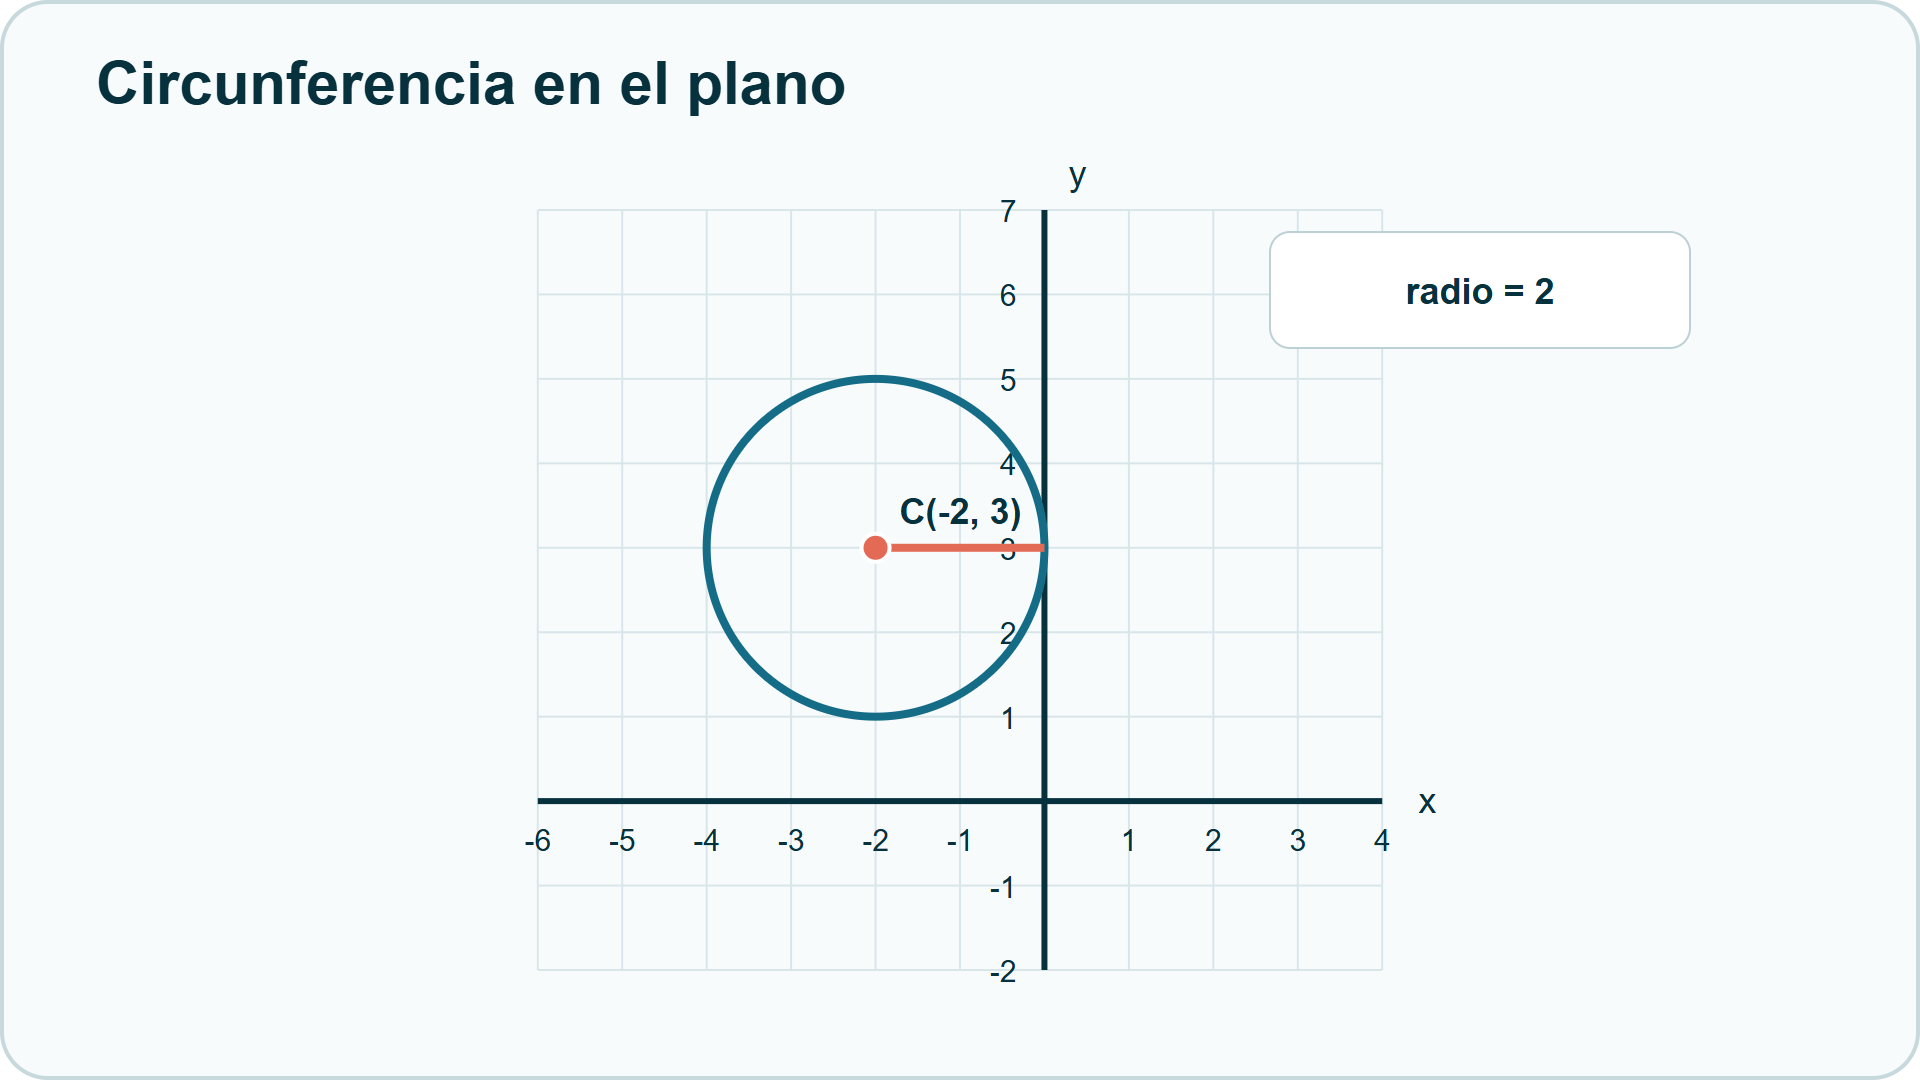
\includegraphics[width=0.80\linewidth,height=0.27\textheight,keepaspectratio]{diagrama-92247cb3b4adc0.png}
\end{center}

\textbf{Respuesta.} $(x+2)^2+(y-3)^2=4$.

\textbf{Pista.} Usa $(x-h)^2+(y-k)^2=r^2$ y cuida los signos del centro.

\textbf{Explicación.} Con $h=-2$, $k=3$ y $r=2$: $(x-(-2))^2+(y-3)^2=2^2$, es decir, $(x+2)^2+(y-3)^2=4$.


\vspace{0.8em}
\hrule
\vspace{1.1em}


\subsection*{\textcolor{DeepBlue}{Circunferencia} \hfill \$200}
\textbf{Pregunta.} Para $(x-4)^2+(y+1)^2=25$, indica el centro y la medida del radio.

\begin{center}
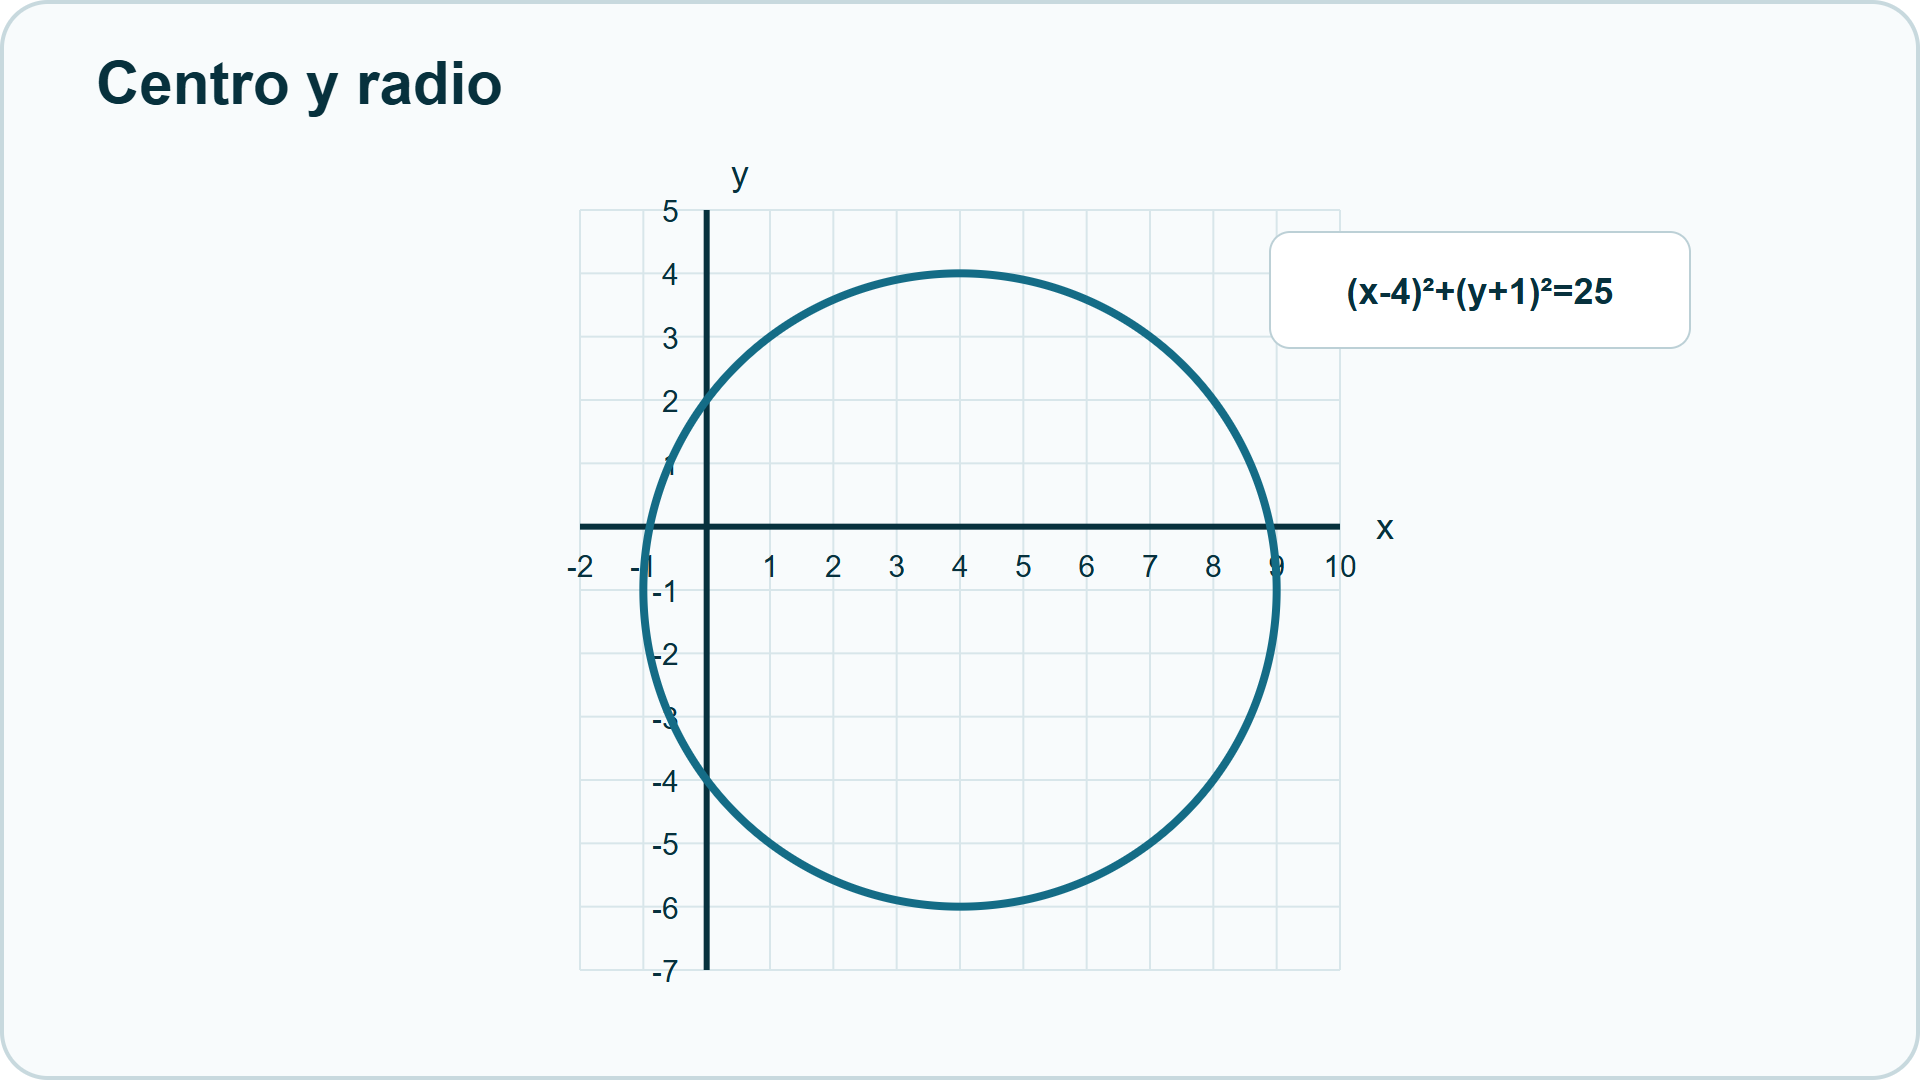
\includegraphics[width=0.80\linewidth,height=0.27\textheight,keepaspectratio]{diagrama-d4dafa80dd8e7d.png}
\end{center}

\textbf{Respuesta.} Centro $(4,-1)$ y radio $5$.

\textbf{Pista.} Compara con $(x-h)^2+(y-k)^2=r^2$.

\textbf{Explicación.} El término $y+1$ es $y-(-1)$, por eso $k=-1$. Además, $r^2=25$, de modo que $r=5$.


\vspace{0.8em}
\hrule
\vspace{1.1em}


\subsection*{\textcolor{DeepBlue}{Circunferencia} \hfill \$300}
\textbf{Pregunta.} La circunferencia $(x-1)^2+(y+2)^2=9$ se traslada $4$ unidades a la izquierda y $5$ hacia arriba. ¿Cuál es la nueva ecuación?

\begin{center}
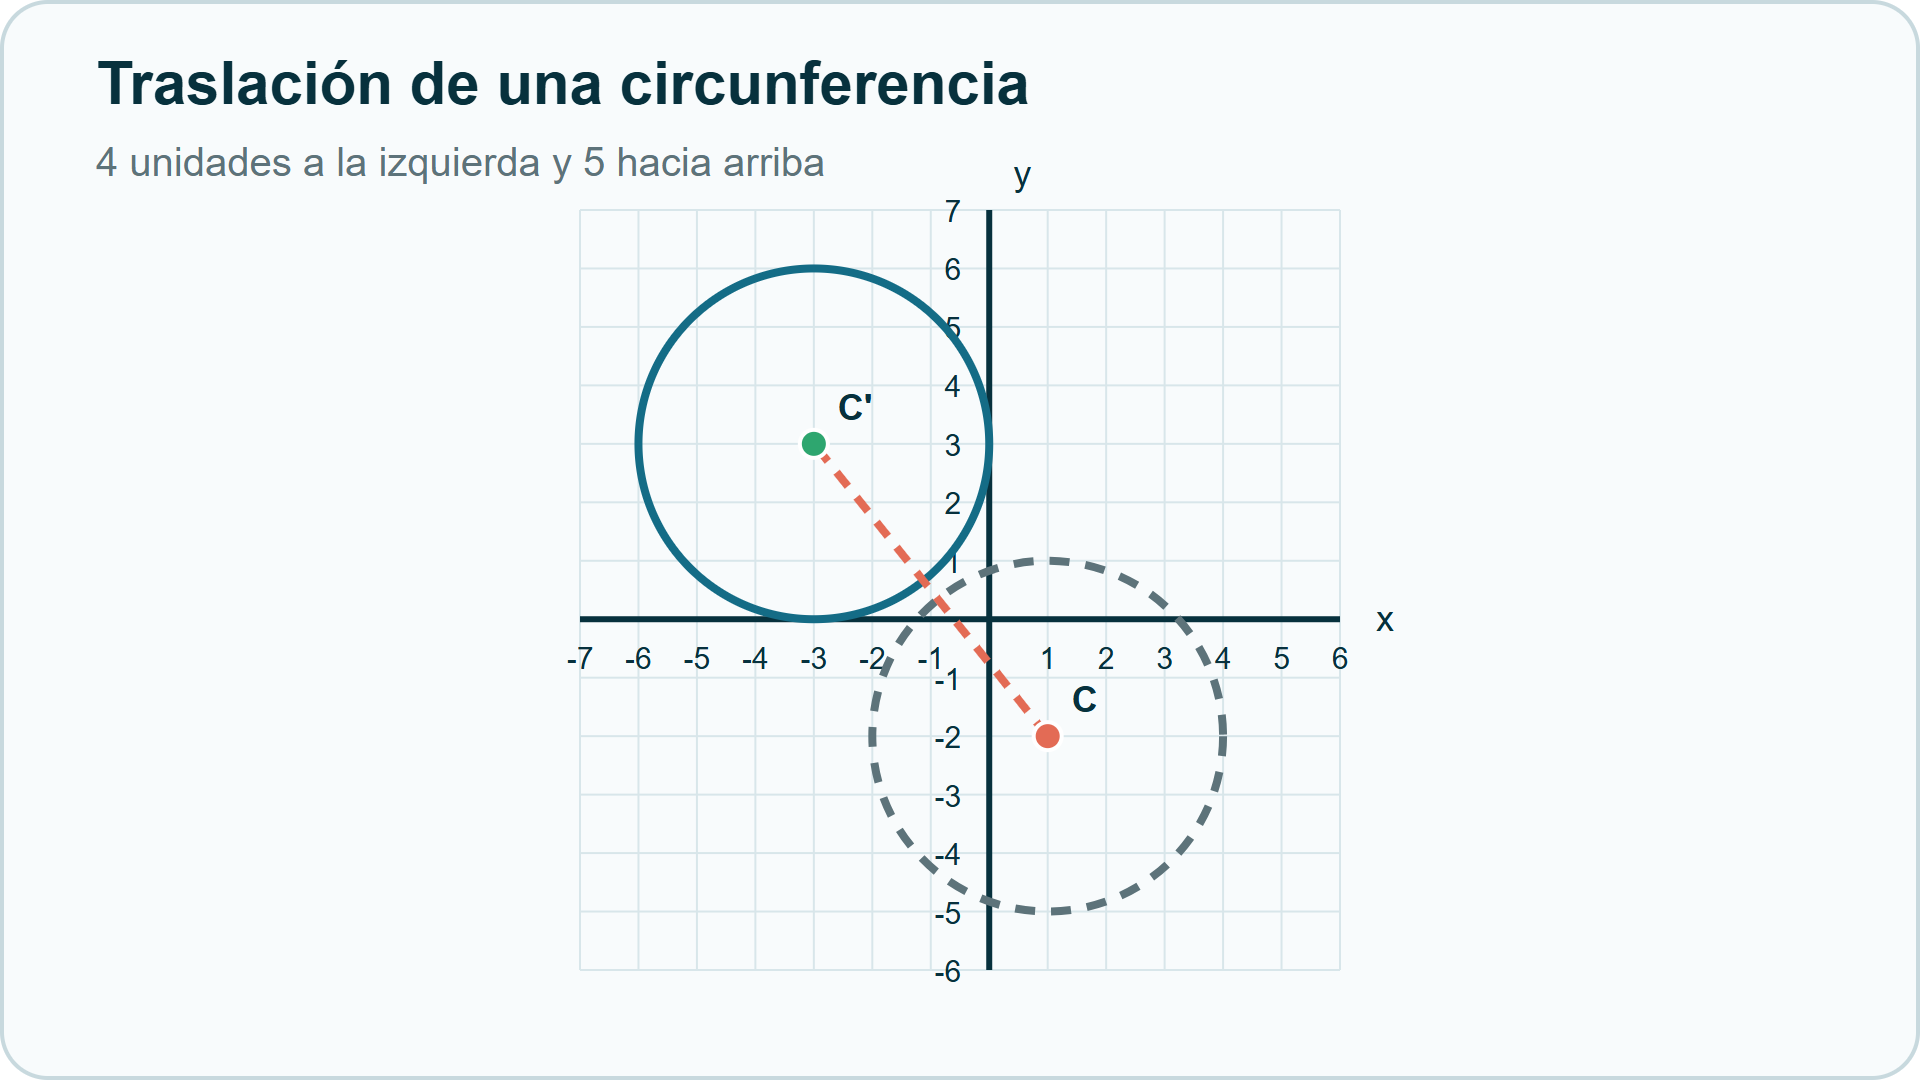
\includegraphics[width=0.80\linewidth,height=0.27\textheight,keepaspectratio]{diagrama-c457ef38ab9f02.png}
\end{center}

\textbf{Respuesta.} $(x+3)^2+(y-3)^2=9$.

\textbf{Pista.} Traslada el centro $(1,-2)$; el radio no cambia.

\textbf{Explicación.} El nuevo centro es $(1-4,-2+5)=(-3,3)$ y el radio sigue siendo $3$. Por eso la ecuación es $(x+3)^2+(y-3)^2=9$.


\vspace{0.8em}
\hrule
\vspace{1.1em}


\subsection*{\textcolor{DeepBlue}{Circunferencia} \hfill \$400}
\textbf{Pregunta.} La circunferencia tiene centro $C(1,1)$ y radio $3$. Clasifica el punto $P(5,1)$ como interior, exterior o perteneciente a la circunferencia.


\textbf{Respuesta.} $P$ es exterior.

\textbf{Pista.} Compara la distancia $CP$ con el radio.

\textbf{Explicación.} $CP=\sqrt{(5-1)^2+(1-1)^2}=4$. Como $4>3$, el punto está fuera de la circunferencia.

\begin{center}
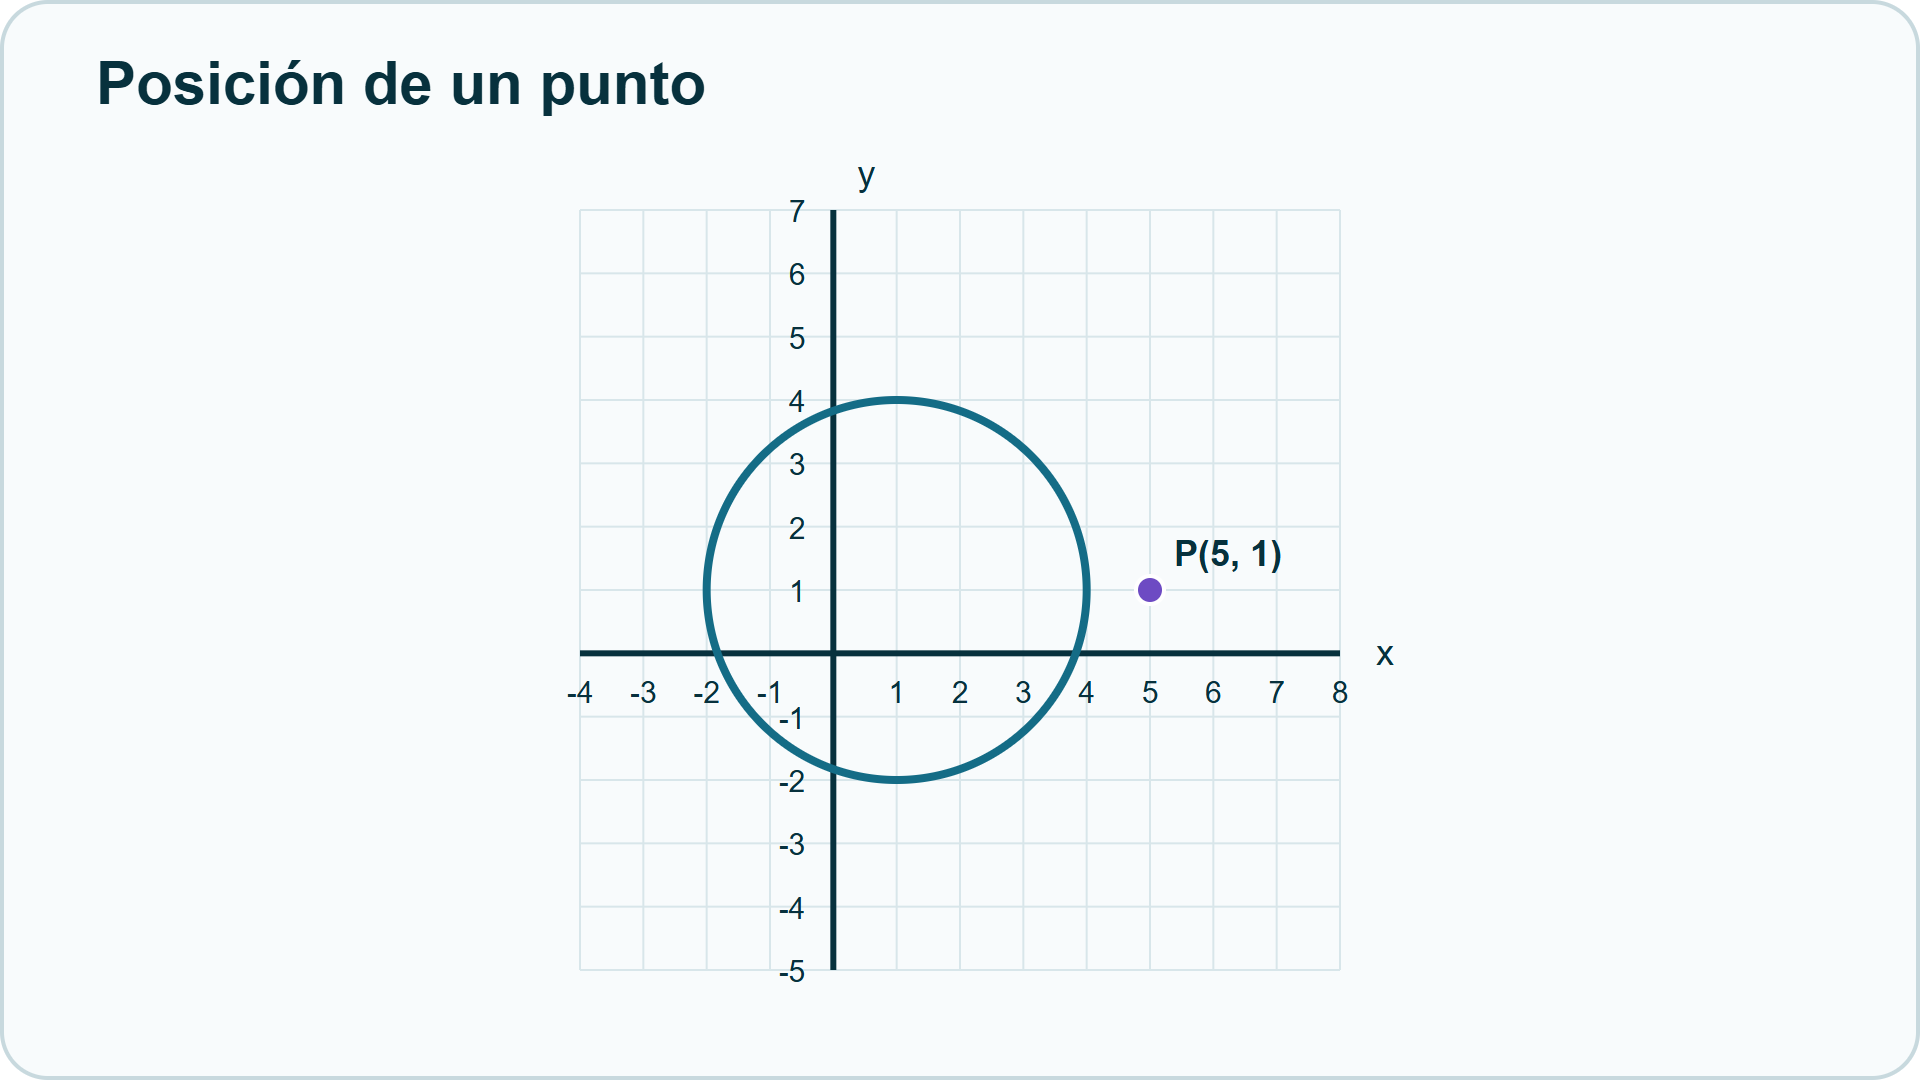
\includegraphics[width=0.80\linewidth,height=0.27\textheight,keepaspectratio]{diagrama-5a990c42c82c85.png}
\end{center}

\vspace{0.8em}
\hrule
\vspace{1.1em}


\subsection*{\textcolor{DeepBlue}{Circunferencia} \hfill \$500}
\textbf{Pregunta.} Una circunferencia tiene centro $C(2,-1)$ y radio $4$. En el punto $Q(6,-1)$ se traza una tangente. ¿Cuál es la ecuación de esa recta?

\begin{center}
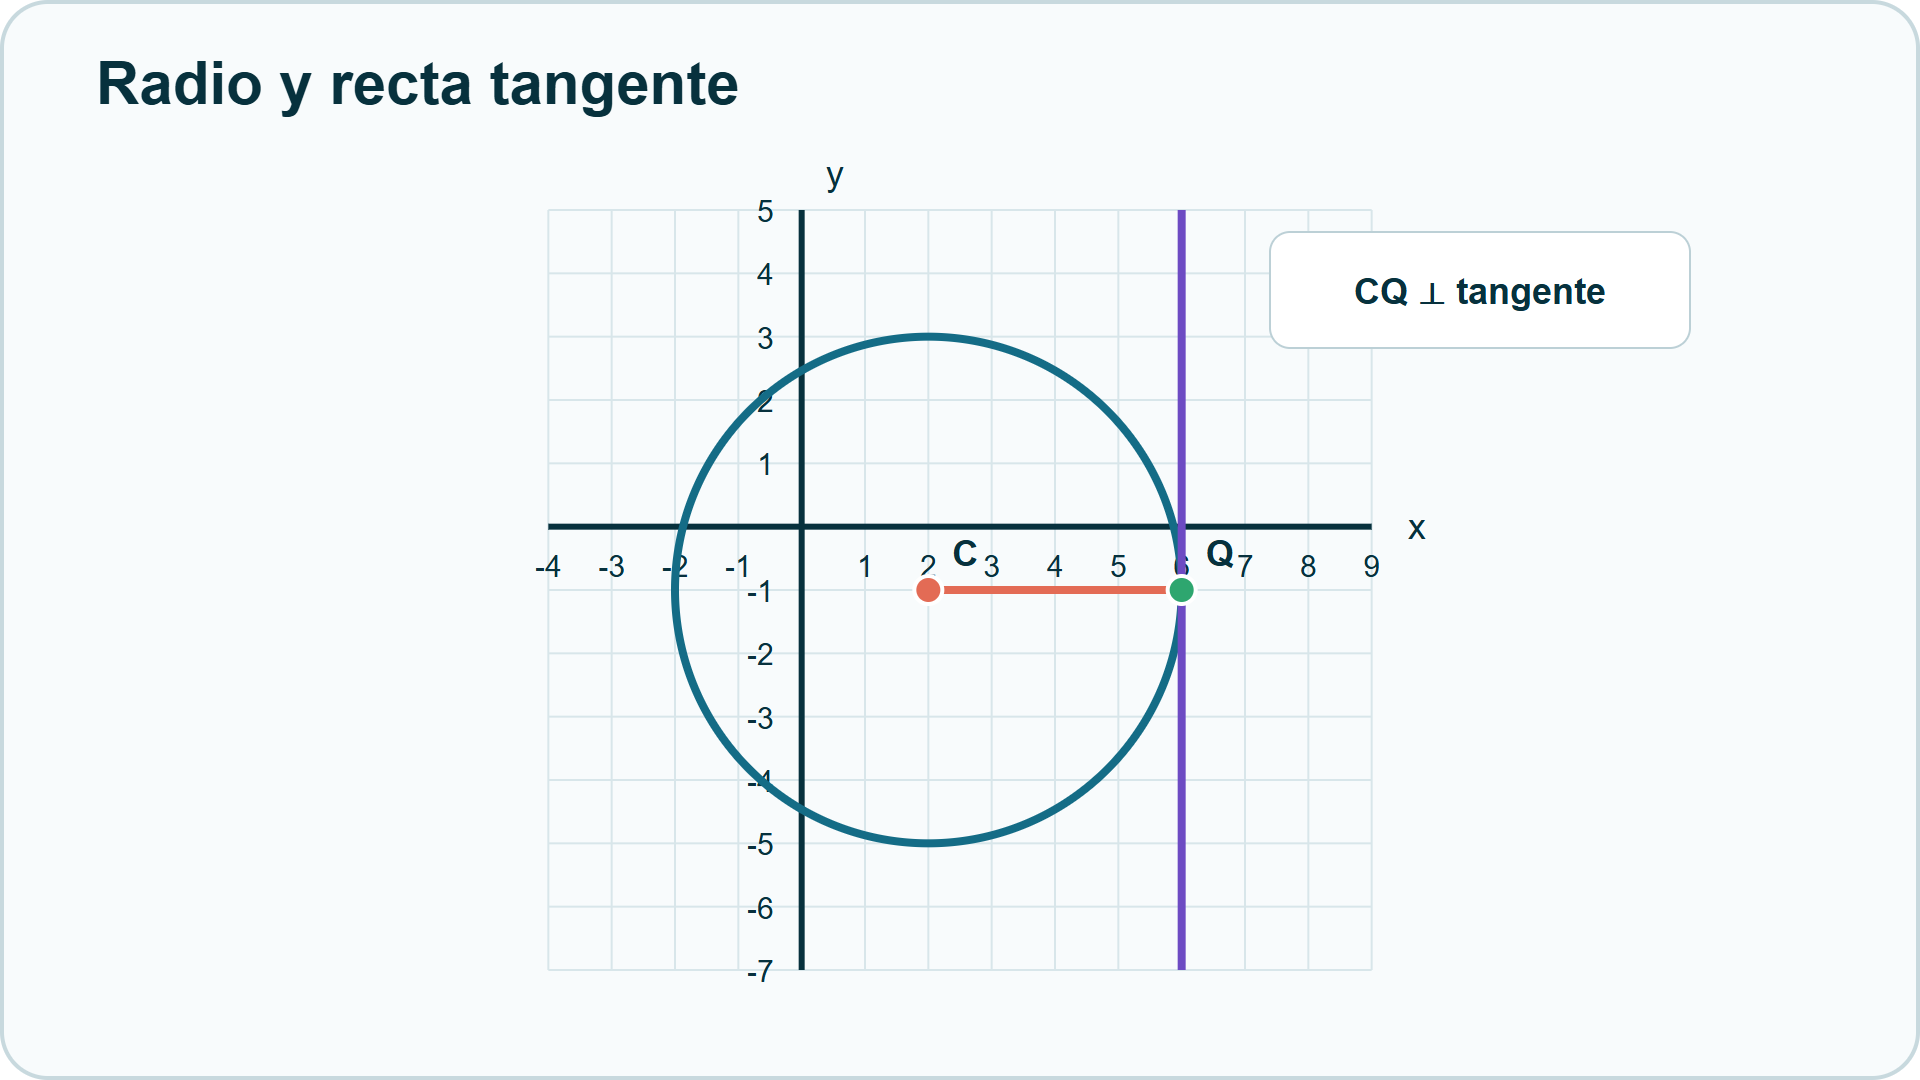
\includegraphics[width=0.80\linewidth,height=0.27\textheight,keepaspectratio]{diagrama-904a63eb7585e3.png}
\end{center}

\textbf{Respuesta.} $x=6$.

\textbf{Pista.} El radio $CQ$ es horizontal; la tangente debe ser perpendicular.

\textbf{Explicación.} El segmento $CQ$ está sobre $y=-1$, por lo que es horizontal. La recta perpendicular que pasa por $Q(6,-1)$ es vertical: $x=6$.


\vspace{0.8em}
\hrule
\vspace{1.1em}



\clearpage
\section*{Geometría}
\addcontentsline{toc}{section}{Geometría}

\subsection*{\textcolor{DeepBlue}{Geometría} \hfill \$100}
\textbf{Pregunta.} Un rectángulo mide $8$ m de largo y $5$ m de ancho. ¿Cuál es su perímetro?


\textbf{Respuesta.} $26$ m.

\textbf{Pista.} Suma dos largos y dos anchos.

\textbf{Explicación.} $P=2(8)+2(5)=16+10=26$ m.


\vspace{0.8em}
\hrule
\vspace{1.1em}


\subsection*{\textcolor{DeepBlue}{Geometría} \hfill \$200}
\textbf{Pregunta.} A un rectángulo de $10$ m por $6$ m se le retira una esquina rectangular de $4$ m por $2$ m. ¿Cuál es el área restante?

\begin{center}
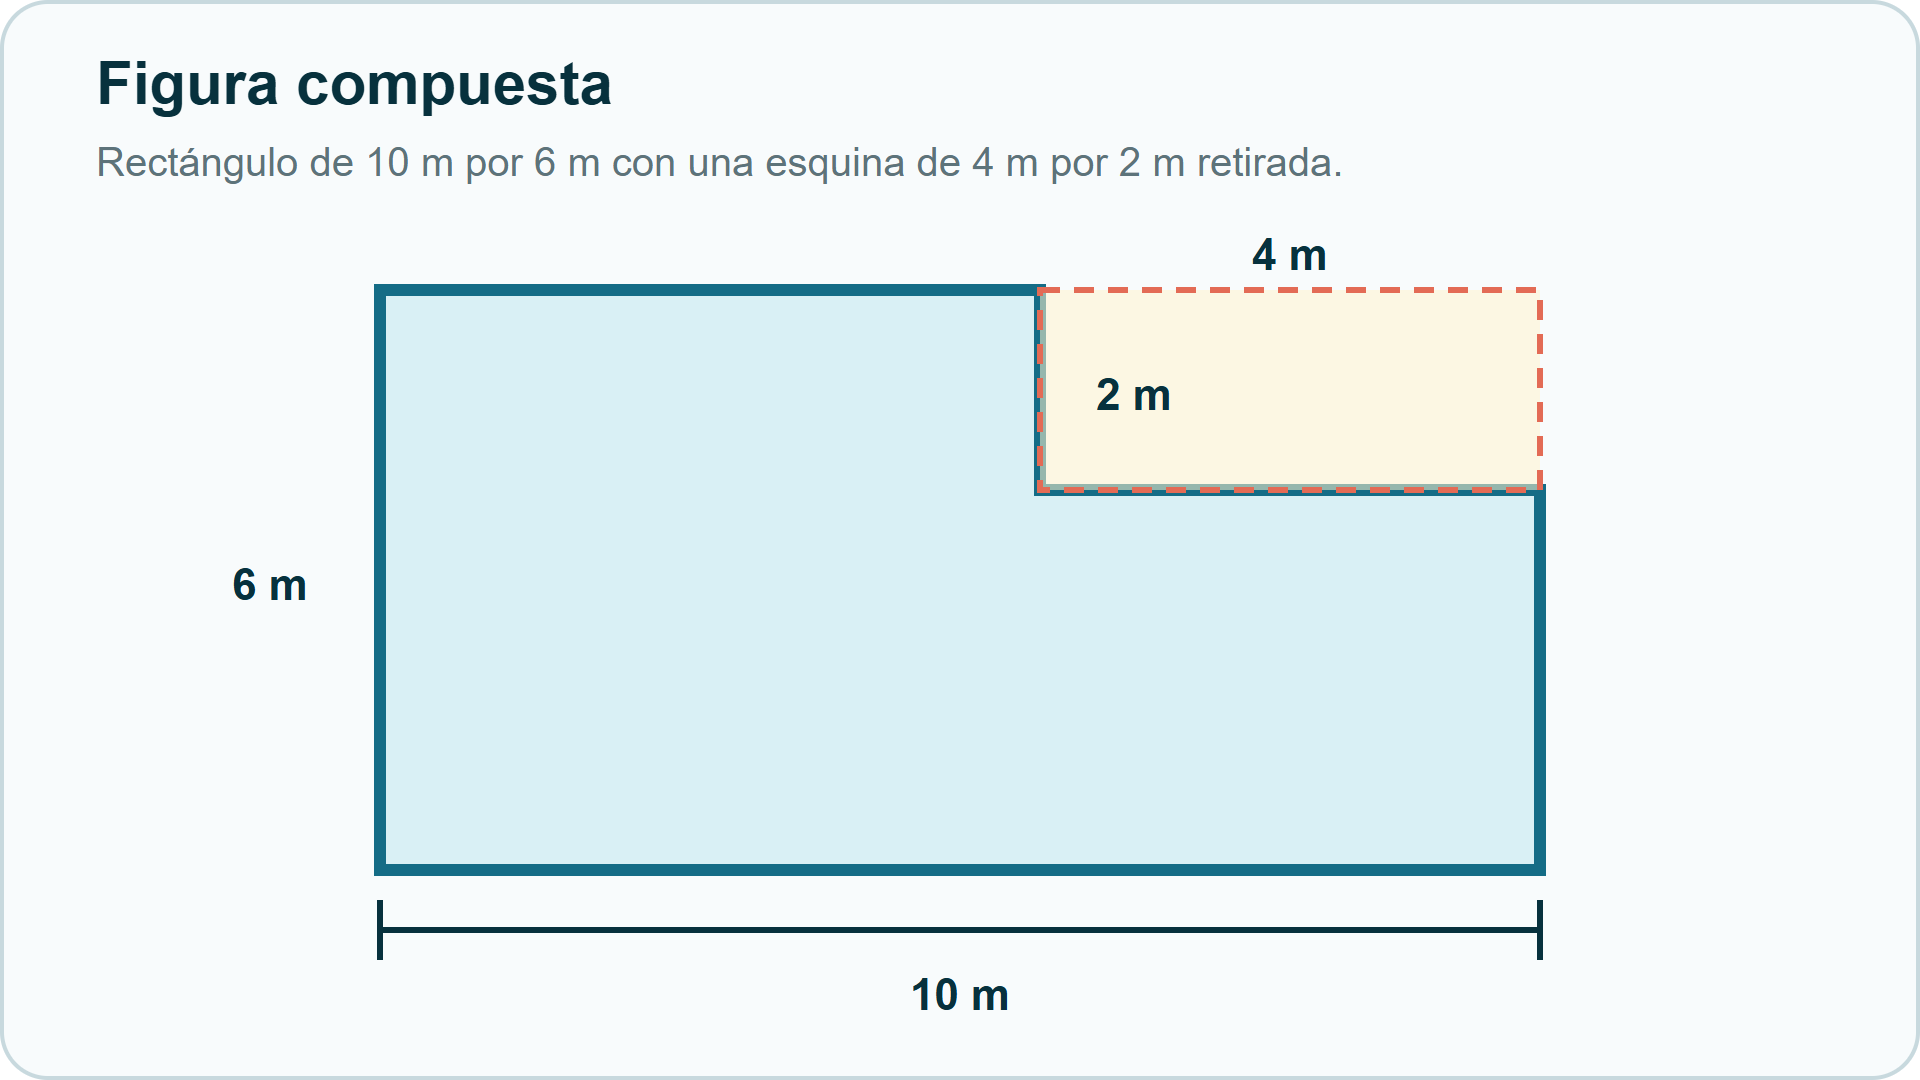
\includegraphics[width=0.80\linewidth,height=0.27\textheight,keepaspectratio]{diagrama-1e3e5b928317e2.png}
\end{center}

\textbf{Respuesta.} $52$ m$^2$.

\textbf{Pista.} Calcula el área grande y resta el área retirada.

\textbf{Explicación.} $10\times6-4\times2=60-8=52$ m$^2$.


\vspace{0.8em}
\hrule
\vspace{1.1em}


\subsection*{\textcolor{DeepBlue}{Geometría} \hfill \$300}
\textbf{Pregunta.} Un cilindro recto tiene radio $3$ cm y altura $8$ cm. Un plano vertical que pasa por su eje produce una sección rectangular. ¿Cuál es el área de esa sección?

\begin{center}
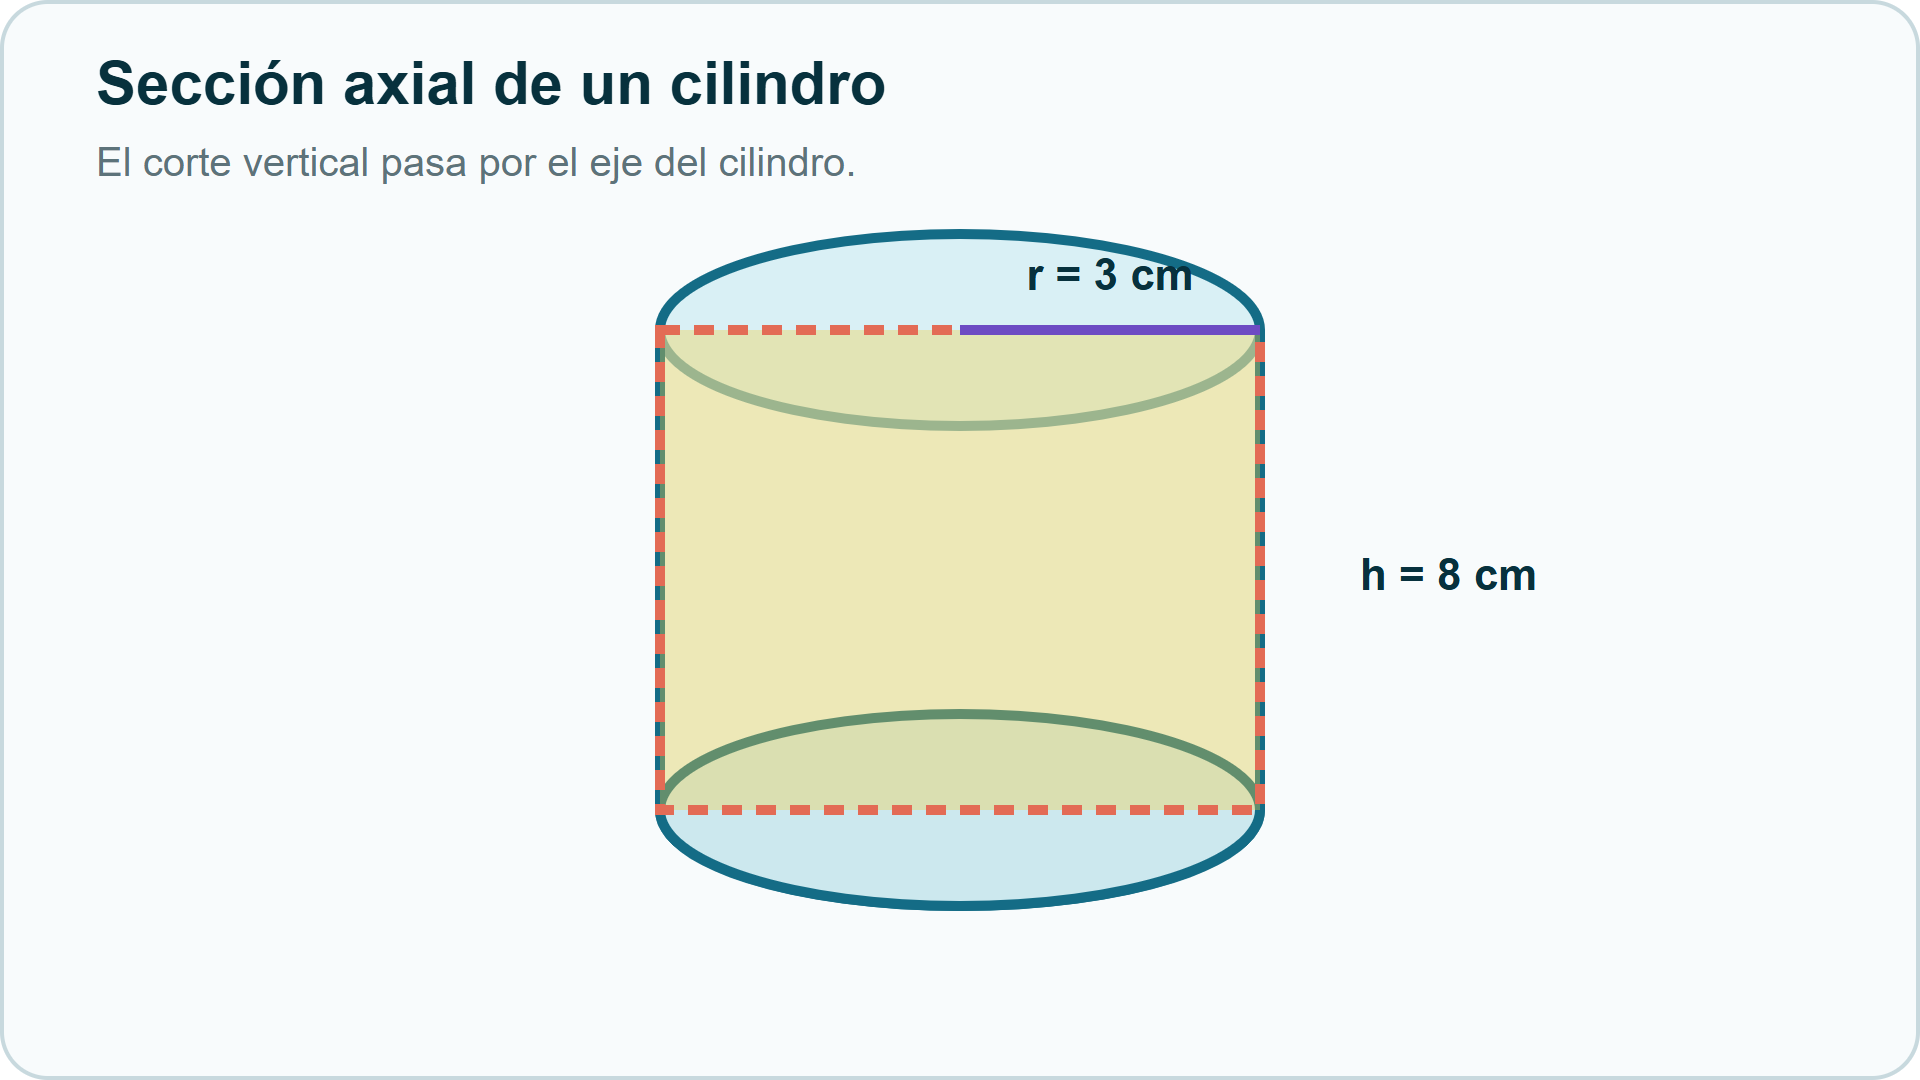
\includegraphics[width=0.80\linewidth,height=0.27\textheight,keepaspectratio]{diagrama-aa2a8d59c35b58.png}
\end{center}

\textbf{Respuesta.} $48$ cm$^2$.

\textbf{Pista.} La base del rectángulo es el diámetro del cilindro.

\textbf{Explicación.} El diámetro es $2r=6$ cm y la altura es $8$ cm. Por tanto, el área de la sección es $6\times8=48$ cm$^2$.


\vspace{0.8em}
\hrule
\vspace{1.1em}


\subsection*{\textcolor{DeepBlue}{Geometría} \hfill \$400}
\textbf{Pregunta.} Refleja el punto $A(-3,2)$ respecto a la recta $y=x$.

\begin{center}
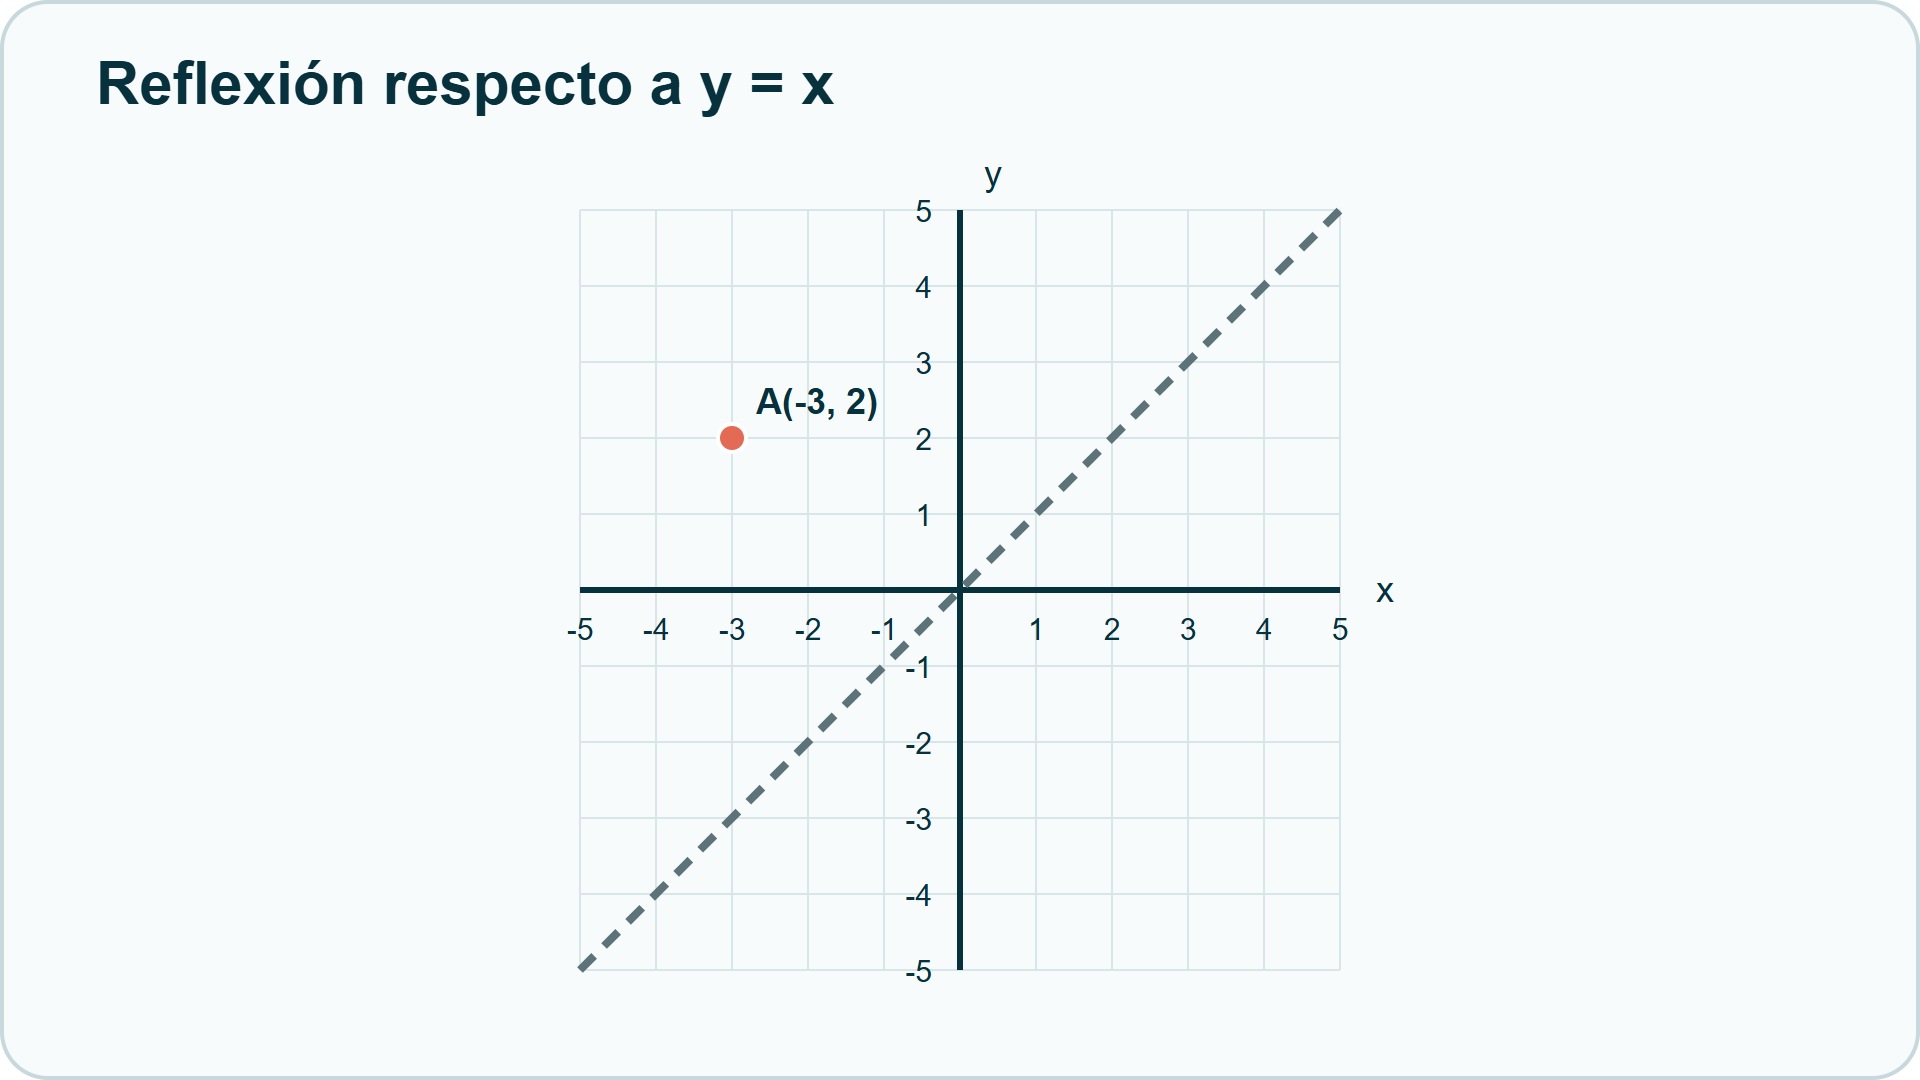
\includegraphics[width=0.80\linewidth,height=0.27\textheight,keepaspectratio]{diagrama-5a7c588387783e.png}
\end{center}

\textbf{Respuesta.} $A'(2,-3)$.

\textbf{Pista.} Al reflejar respecto a $y=x$, se intercambian las coordenadas.

\textbf{Explicación.} La regla es $(x,y)\mapsto(y,x)$. Así, $(-3,2)\mapsto(2,-3)$.

\begin{center}
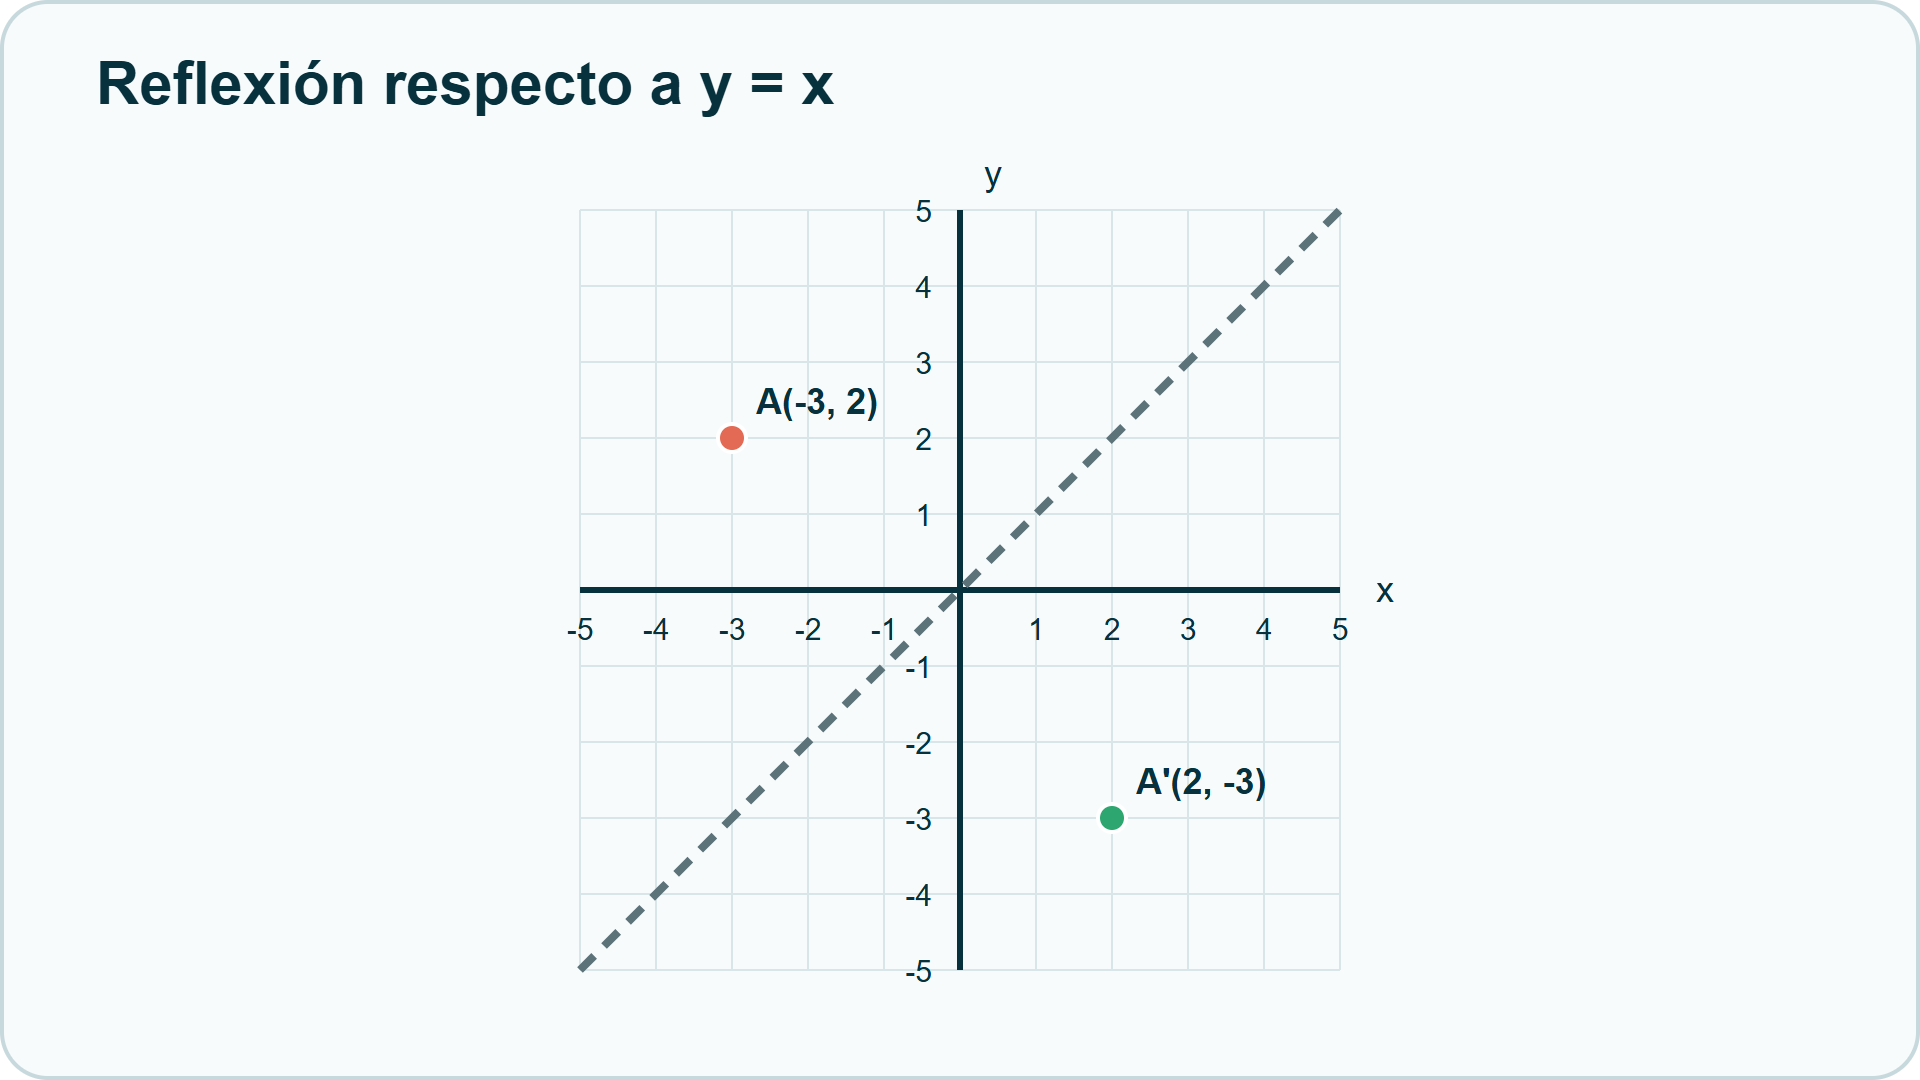
\includegraphics[width=0.80\linewidth,height=0.27\textheight,keepaspectratio]{diagrama-40e87a14cdd89e.png}
\end{center}

\vspace{0.8em}
\hrule
\vspace{1.1em}


\subsection*{\textcolor{DeepBlue}{Geometría} \hfill \$500}
\textbf{Pregunta.} Aplica al triángulo $A(1,1)$, $B(4,1)$, $C(1,3)$ una homotecia de centro en el origen y razón $k=-2$.

\begin{center}
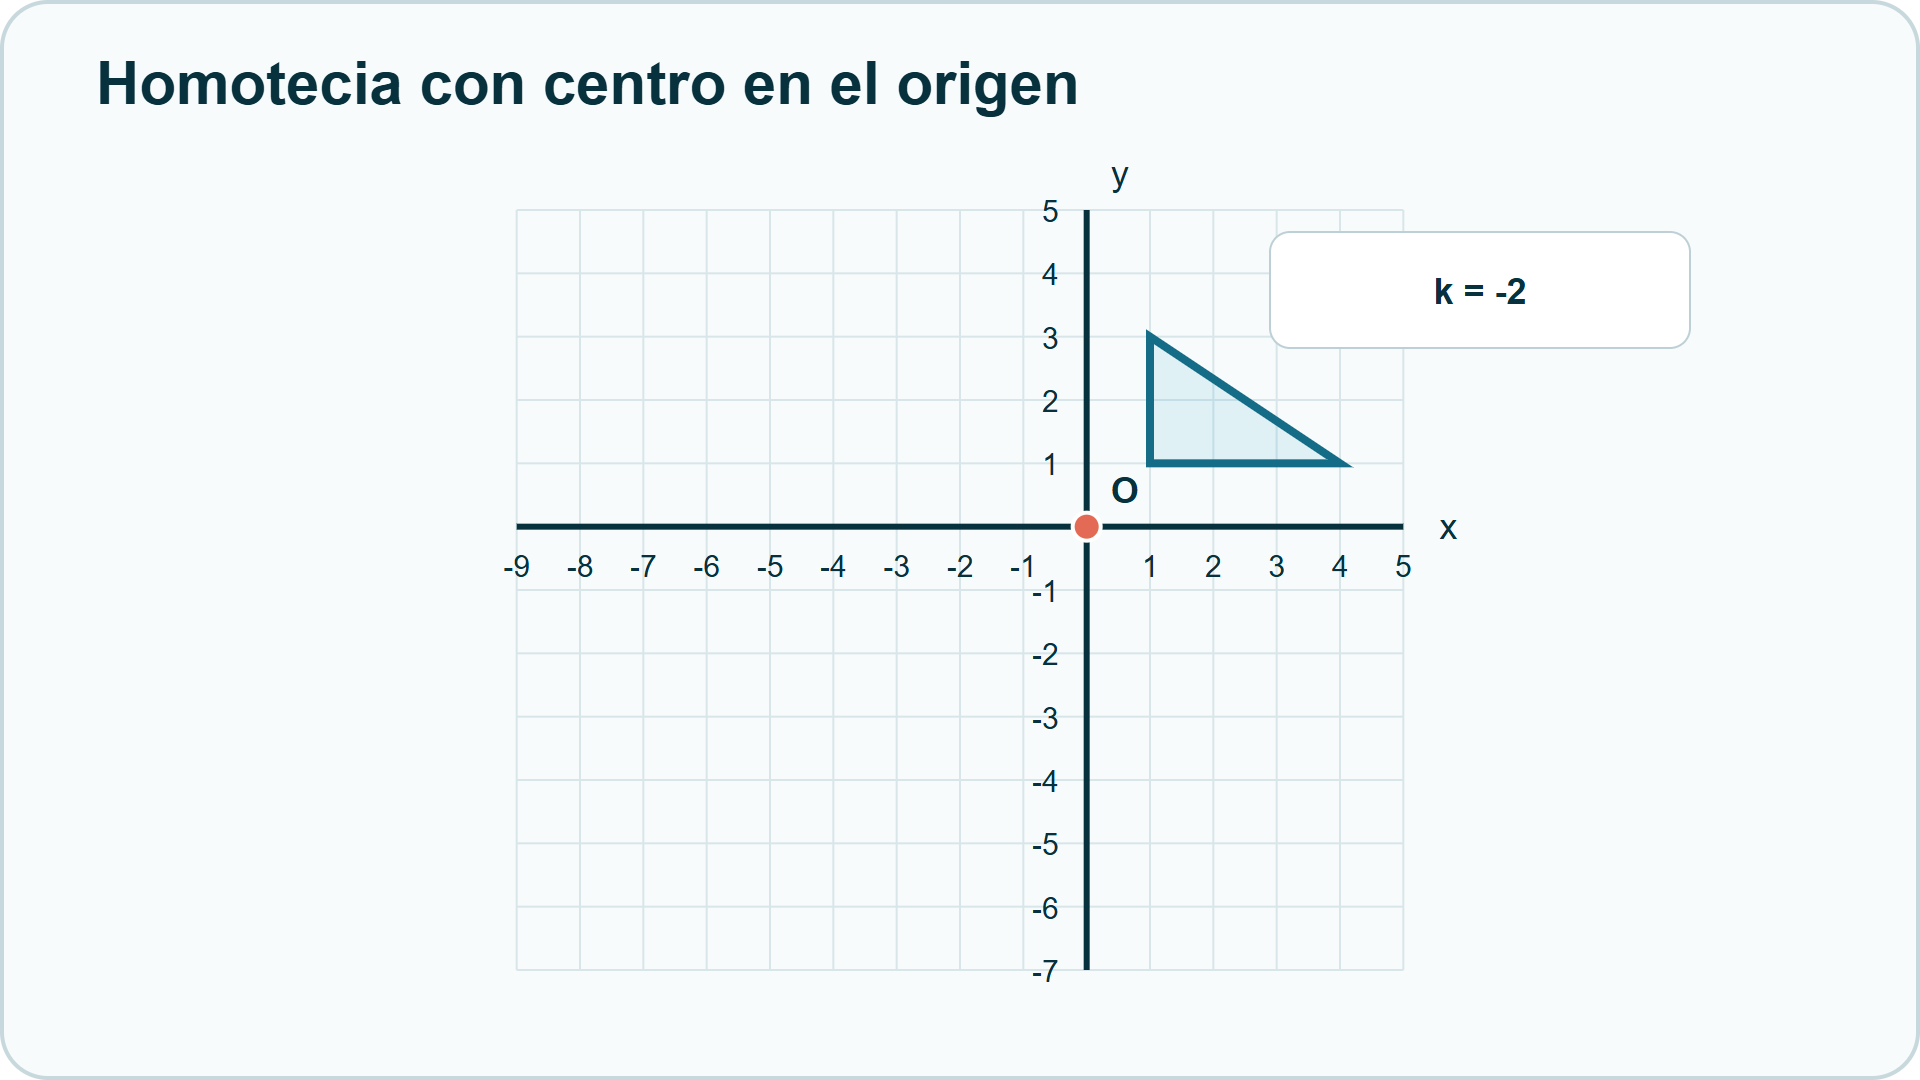
\includegraphics[width=0.80\linewidth,height=0.27\textheight,keepaspectratio]{diagrama-0047472fe0aa86.png}
\end{center}

\textbf{Respuesta.} $A'(-2,-2)$, $B'(-8,-2)$ y $C'(-2,-6)$.

\textbf{Pista.} Multiplica cada coordenada por $-2$.

\textbf{Explicación.} En una homotecia centrada en el origen, $(x,y)\mapsto(kx,ky)$. El signo negativo coloca la imagen al lado opuesto y el factor $2$ duplica las distancias.

\begin{center}
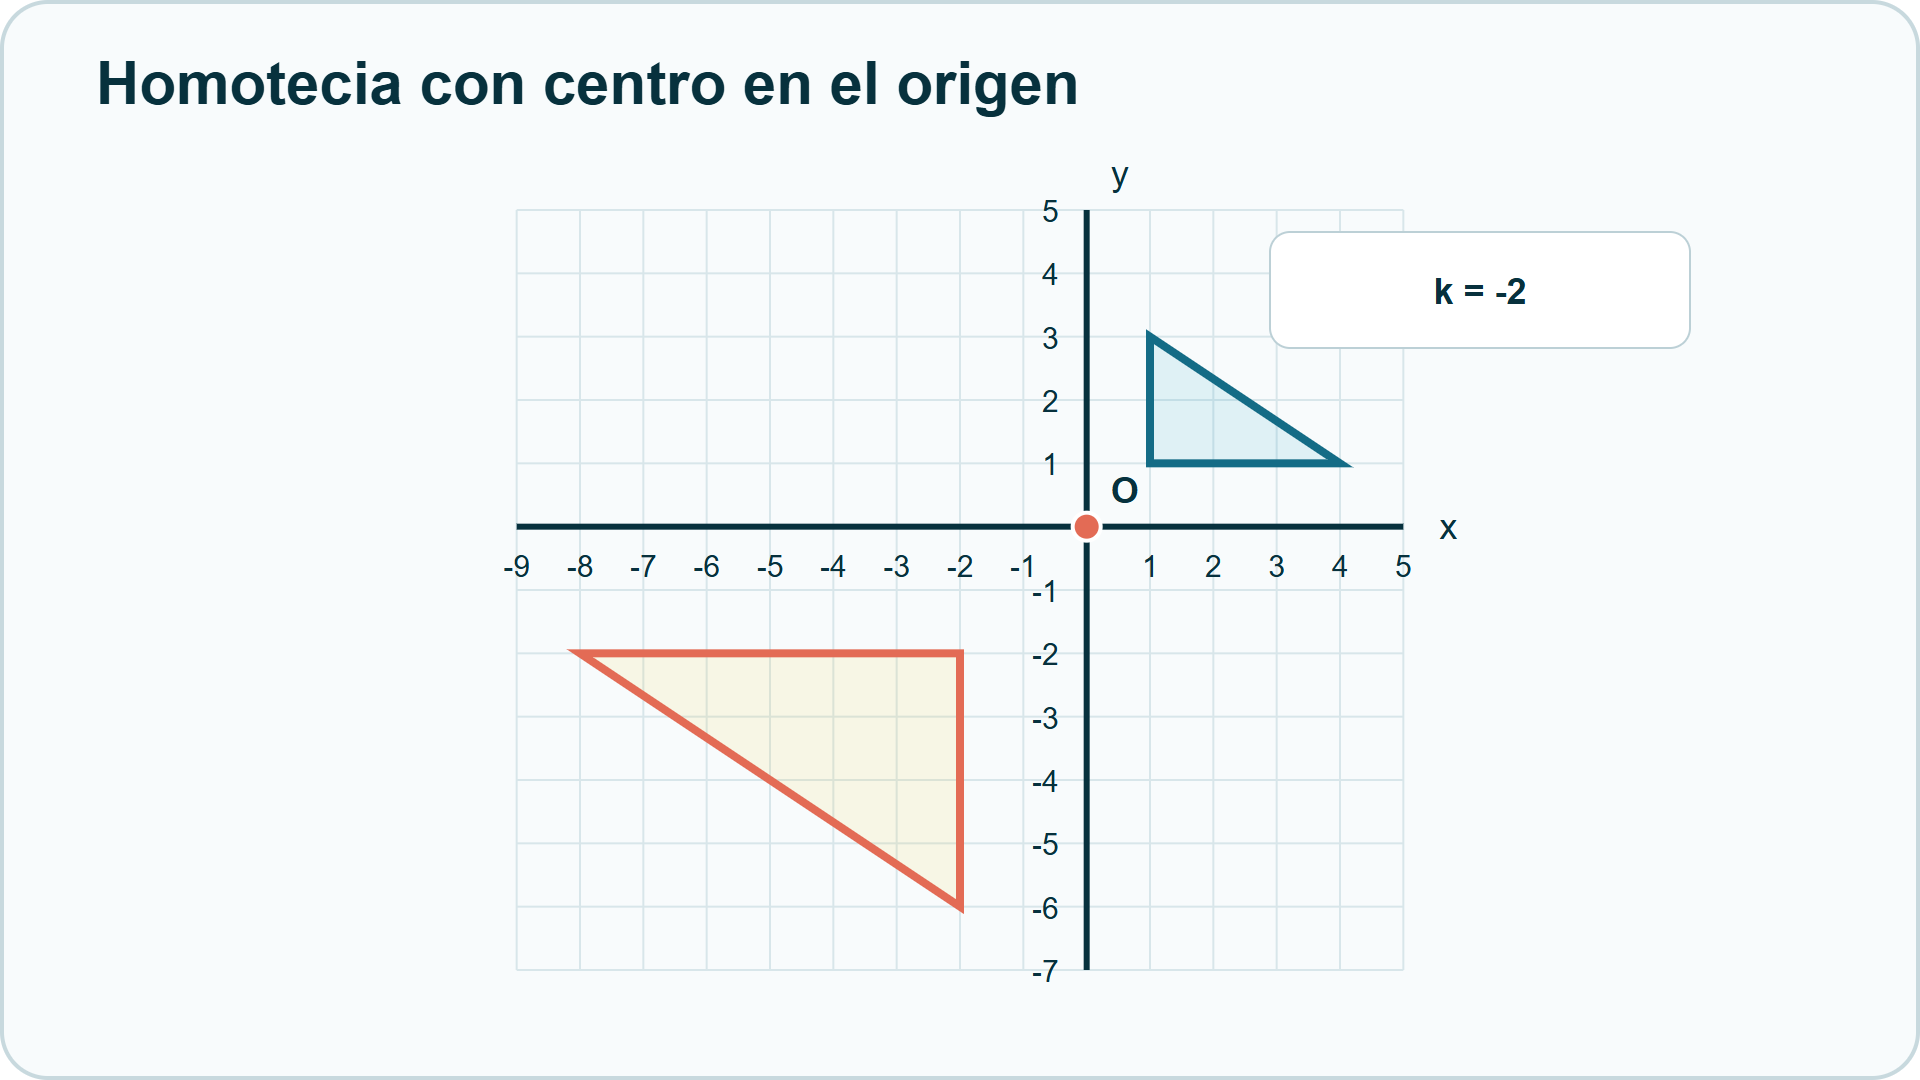
\includegraphics[width=0.80\linewidth,height=0.27\textheight,keepaspectratio]{diagrama-03f2709e760af1.png}
\end{center}

\vspace{0.8em}
\hrule
\vspace{1.1em}



\clearpage
\section*{Funciones}
\addcontentsline{toc}{section}{Funciones}

\subsection*{\textcolor{DeepBlue}{Funciones} \hfill \$100}
\textbf{Pregunta.} Según el diagrama, ¿la relación representada es una función? Justifica.

\begin{center}
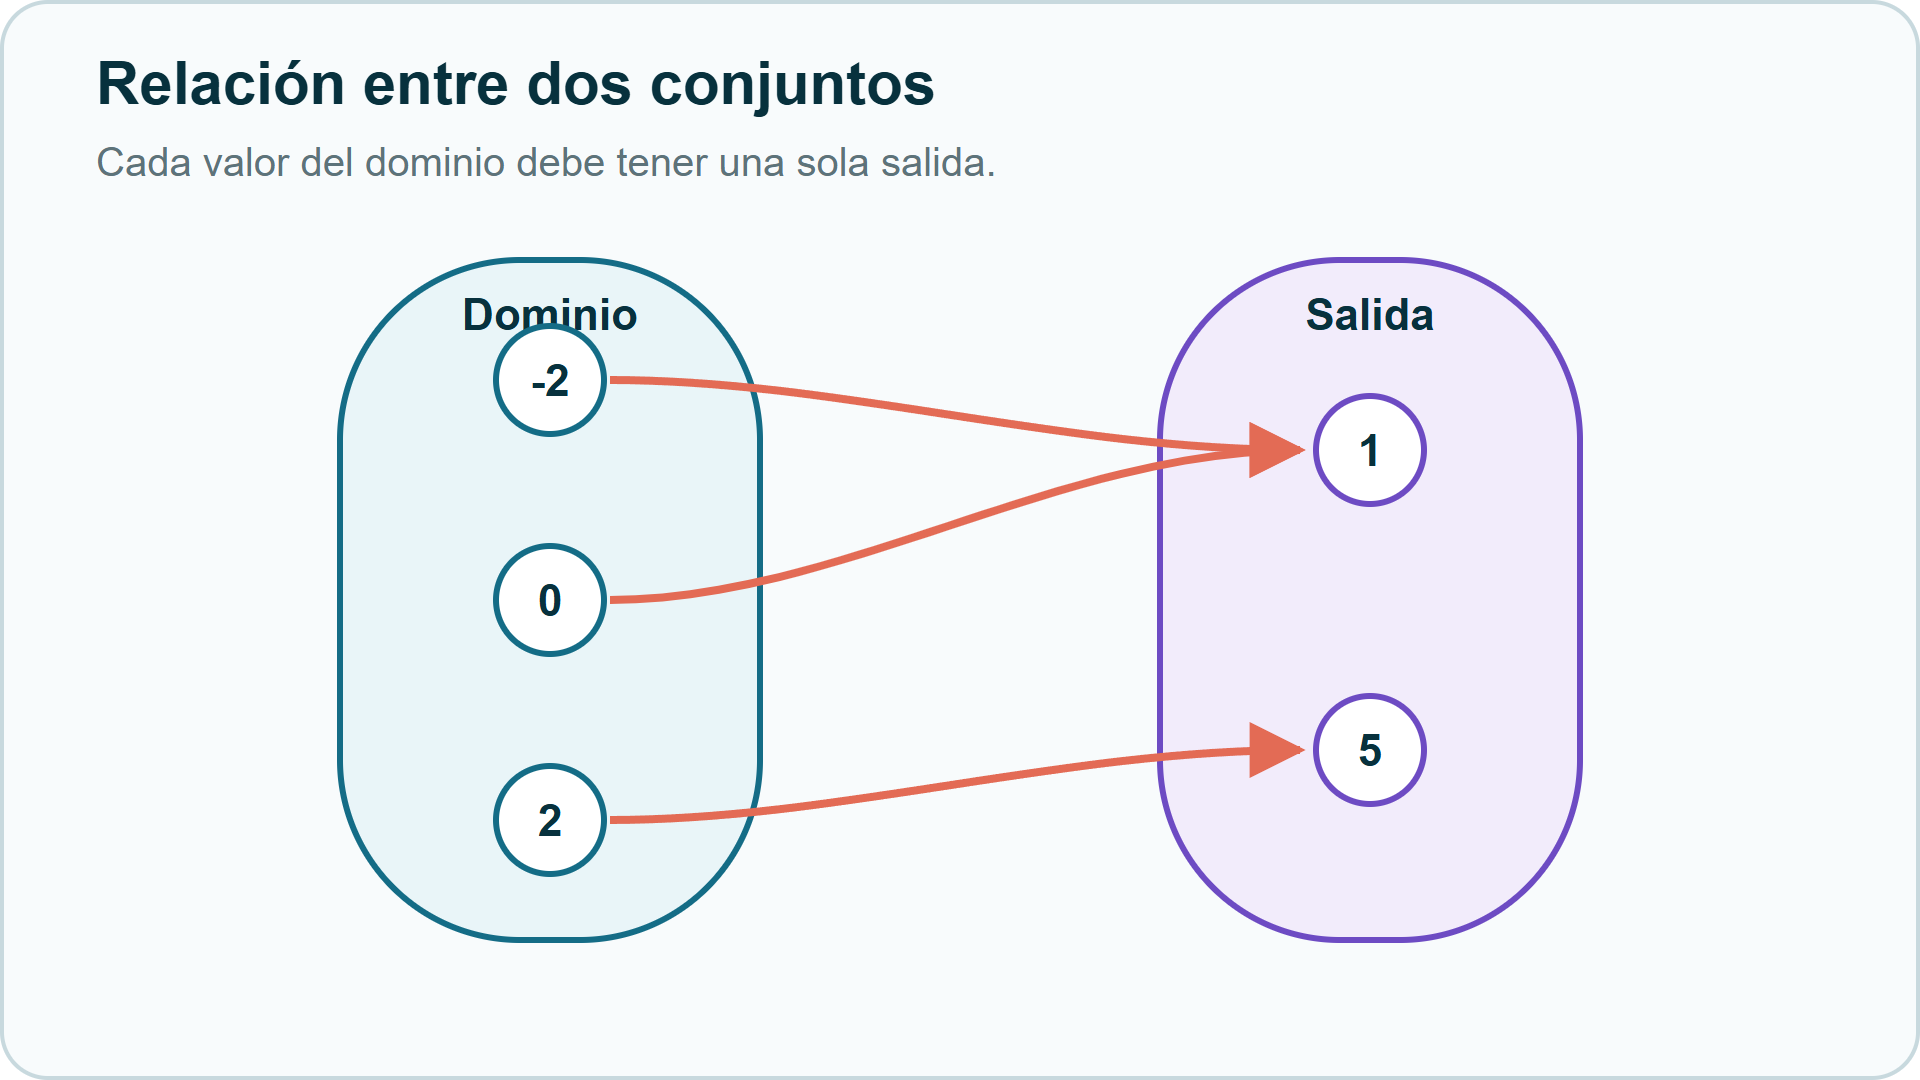
\includegraphics[width=0.80\linewidth,height=0.27\textheight,keepaspectratio]{diagrama-8a95d9fe760ce8.png}
\end{center}

\textbf{Respuesta.} Sí. Cada elemento del dominio tiene exactamente una salida.

\textbf{Pista.} Revisa cuántas flechas salen de cada valor del dominio.

\textbf{Explicación.} Aunque $-2$ y $0$ tienen la misma imagen, esto sí se permite. Lo importante es que de cada entrada salga una sola flecha.


\vspace{0.8em}
\hrule
\vspace{1.1em}


\subsection*{\textcolor{DeepBlue}{Funciones} \hfill \$200}
\textbf{Pregunta.} Una recta pasa por $(2,5)$ y $(6,13)$. Determina su pendiente y su ecuación.

\begin{center}
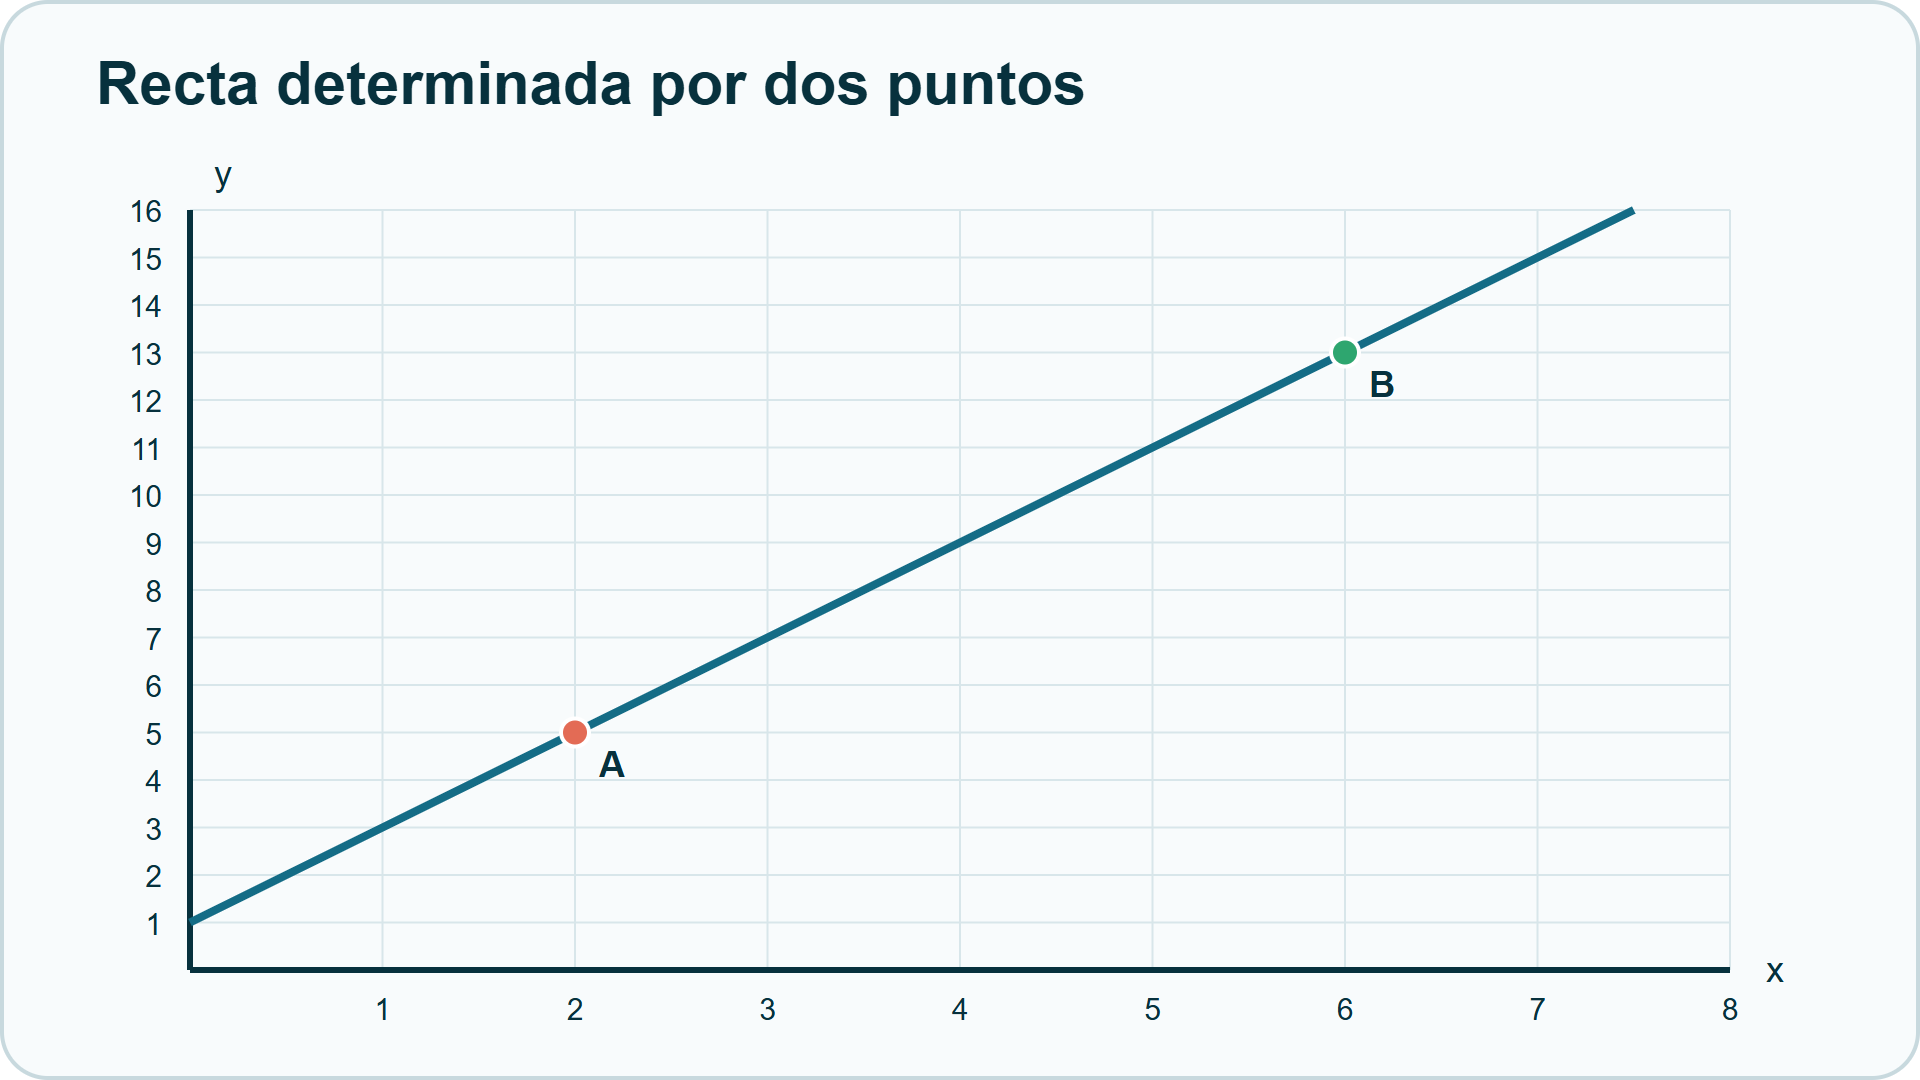
\includegraphics[width=0.80\linewidth,height=0.27\textheight,keepaspectratio]{diagrama-659de0813143d9.png}
\end{center}

\textbf{Respuesta.} Pendiente $m=2$; ecuación $y=2x+1$.

\textbf{Pista.} Calcula $m=\frac{13-5}{6-2}$ y luego usa uno de los puntos.

\textbf{Explicación.} $m=\frac{8}{4}=2$. En $y=mx+b$, al usar $(2,5)$: $5=2(2)+b$, de donde $b=1$.


\vspace{0.8em}
\hrule
\vspace{1.1em}


\subsection*{\textcolor{DeepBlue}{Funciones} \hfill \$300}
\textbf{Pregunta.} Para $f(x)=-(x-3)^2+4$, indica el valor máximo y los ceros.


\textbf{Respuesta.} Máximo $4$ en $x=3$; ceros $x=1$ y $x=5$.

\textbf{Pista.} La forma de vértice permite leer el máximo. Para los ceros, iguala $f(x)$ a $0$.

\textbf{Explicación.} El vértice es $(3,4)$ y la parábola abre hacia abajo. Al resolver $-(x-3)^2+4=0$, se obtiene $(x-3)^2=4$, por lo que $x=1$ o $x=5$.

\begin{center}
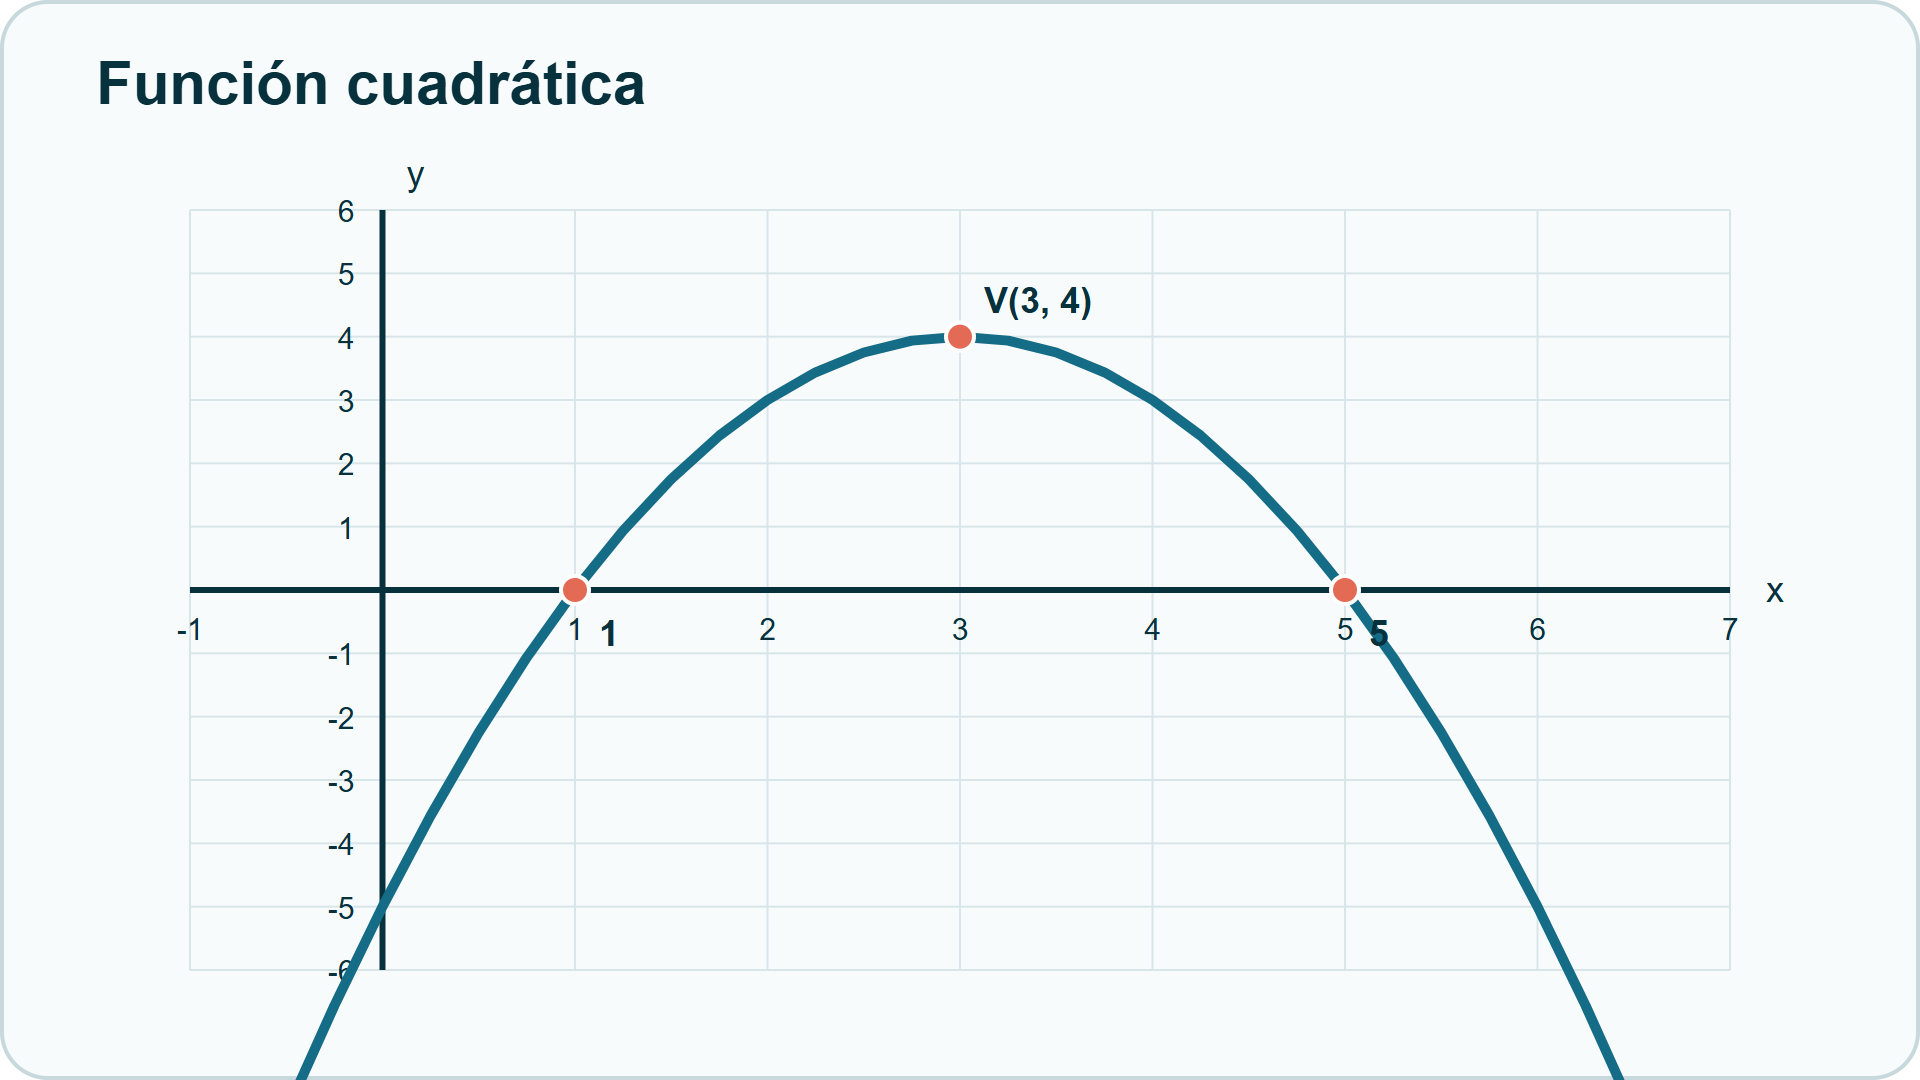
\includegraphics[width=0.80\linewidth,height=0.27\textheight,keepaspectratio]{diagrama-510c6d8b5815f7.png}
\end{center}

\vspace{0.8em}
\hrule
\vspace{1.1em}


\subsection*{\textcolor{DeepBlue}{Funciones} \hfill \$400}
\textbf{Pregunta.} Resuelve el sistema $y=2x+1$ y $y=-x+7$.

\begin{center}
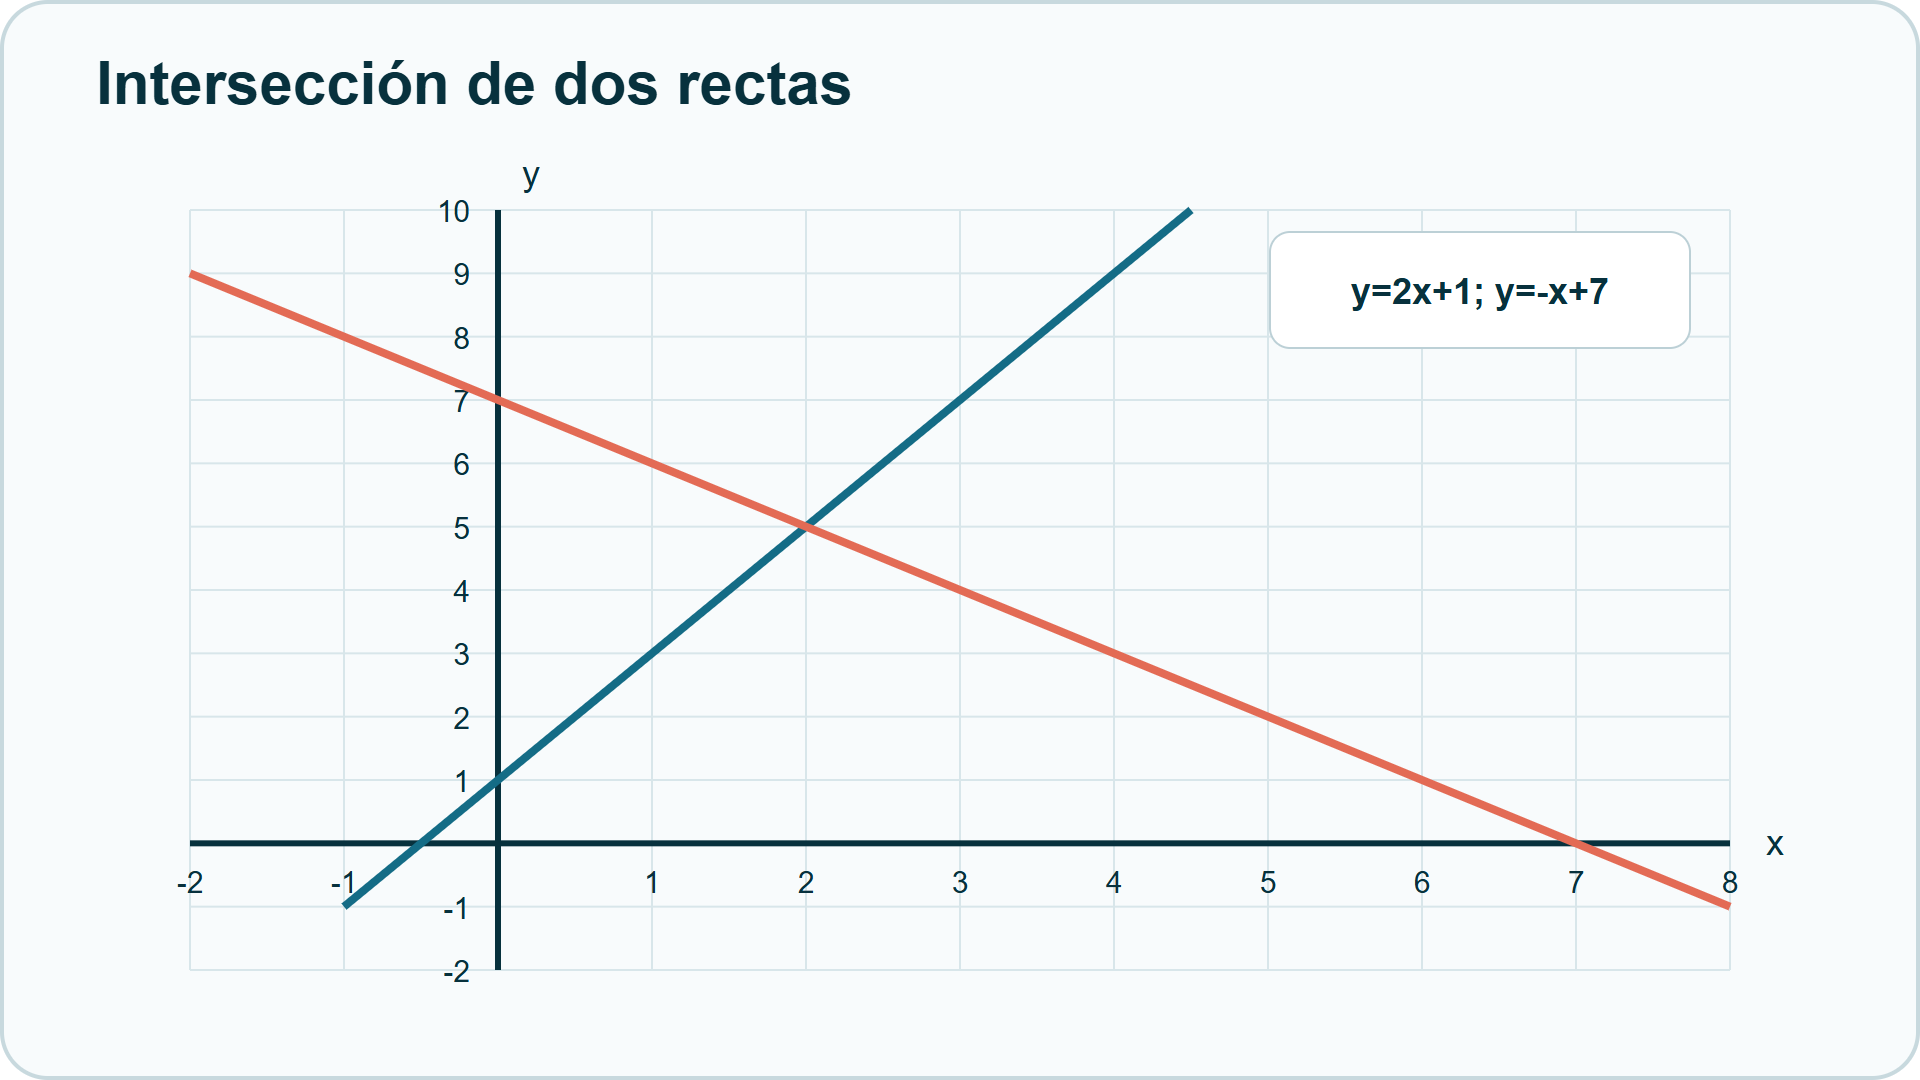
\includegraphics[width=0.80\linewidth,height=0.27\textheight,keepaspectratio]{diagrama-d1870b5eb5295e.png}
\end{center}

\textbf{Respuesta.} $(x,y)=(2,5)$.

\textbf{Pista.} Iguala las dos expresiones de $y$.

\textbf{Explicación.} $2x+1=-x+7$ implica $3x=6$, así que $x=2$. Al sustituir, $y=2(2)+1=5$. Gráficamente, es el punto de intersección.

\begin{center}
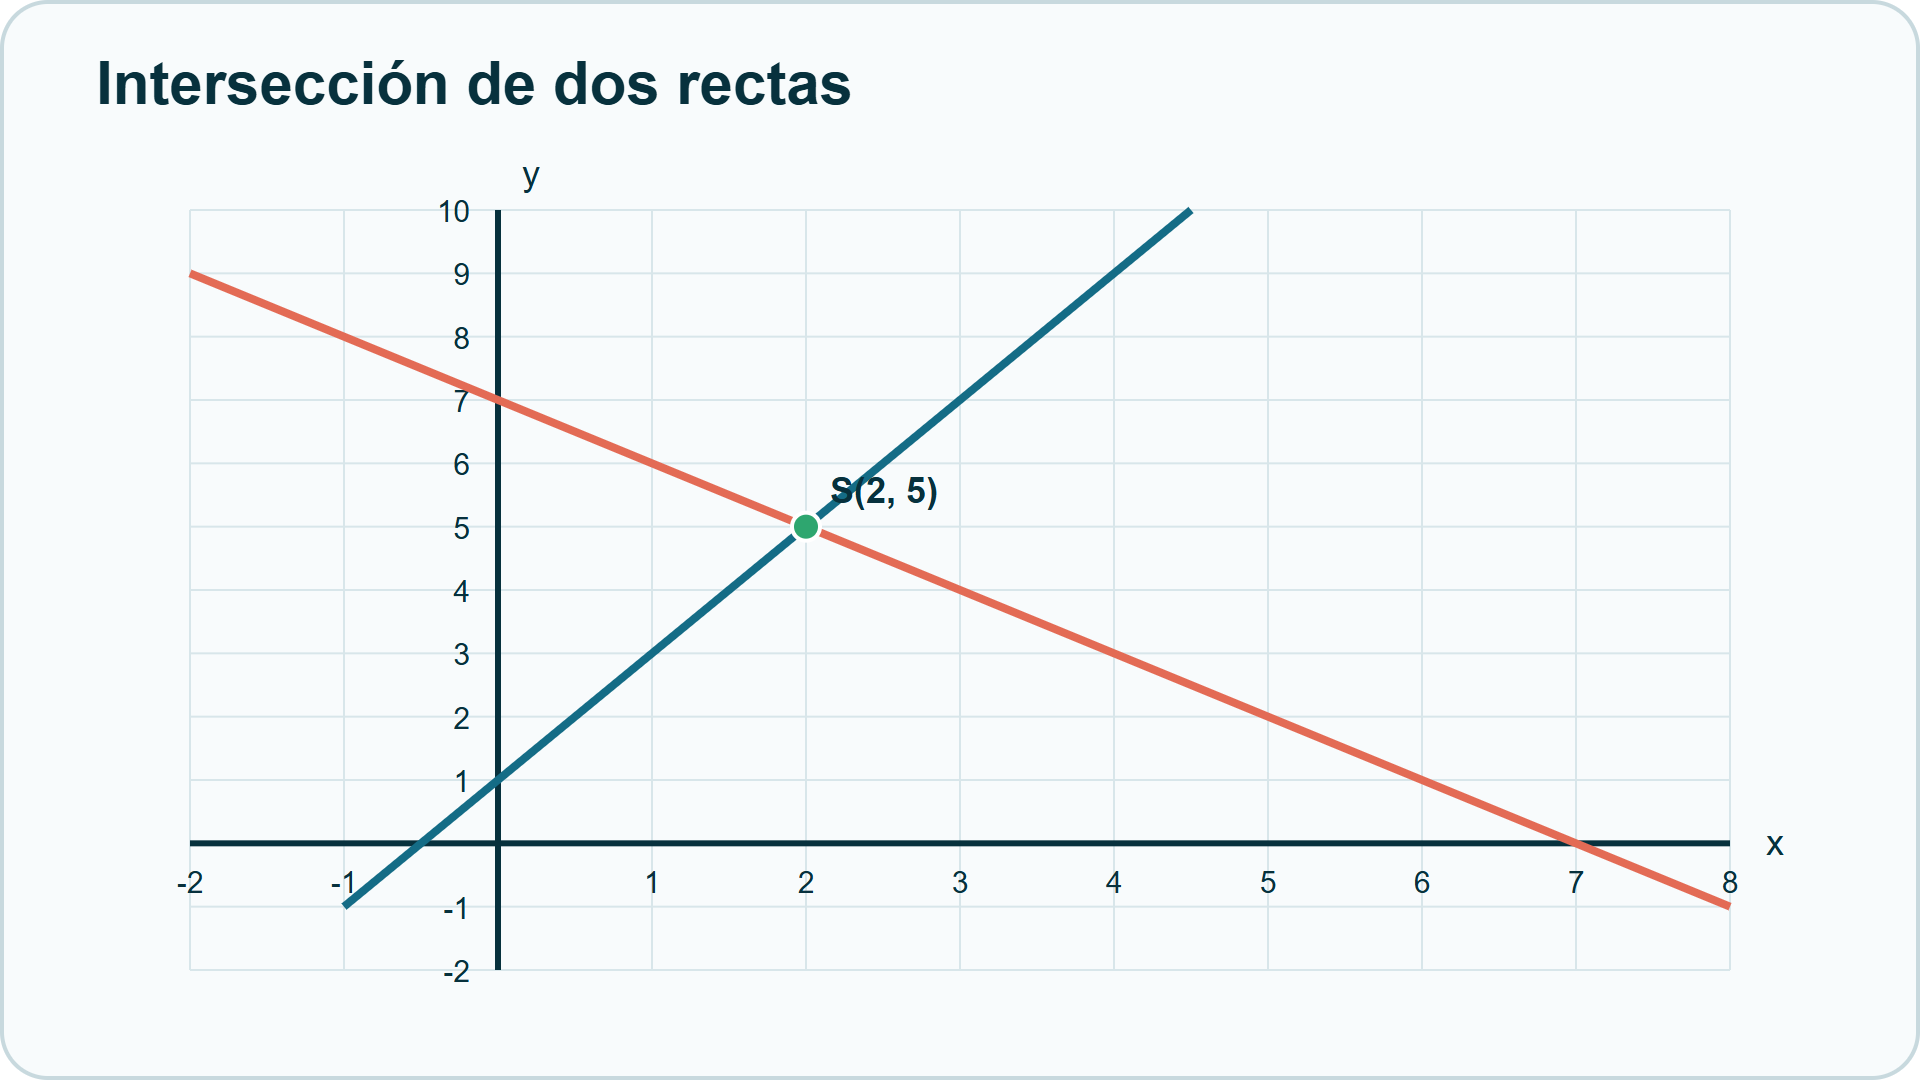
\includegraphics[width=0.80\linewidth,height=0.27\textheight,keepaspectratio]{diagrama-055be0c43455d3.png}
\end{center}

\vspace{0.8em}
\hrule
\vspace{1.1em}


\subsection*{\textcolor{DeepBlue}{Funciones} \hfill \$500}
\textbf{Pregunta.} Determina la inversa de $f(x)=3x-6$.

\begin{center}
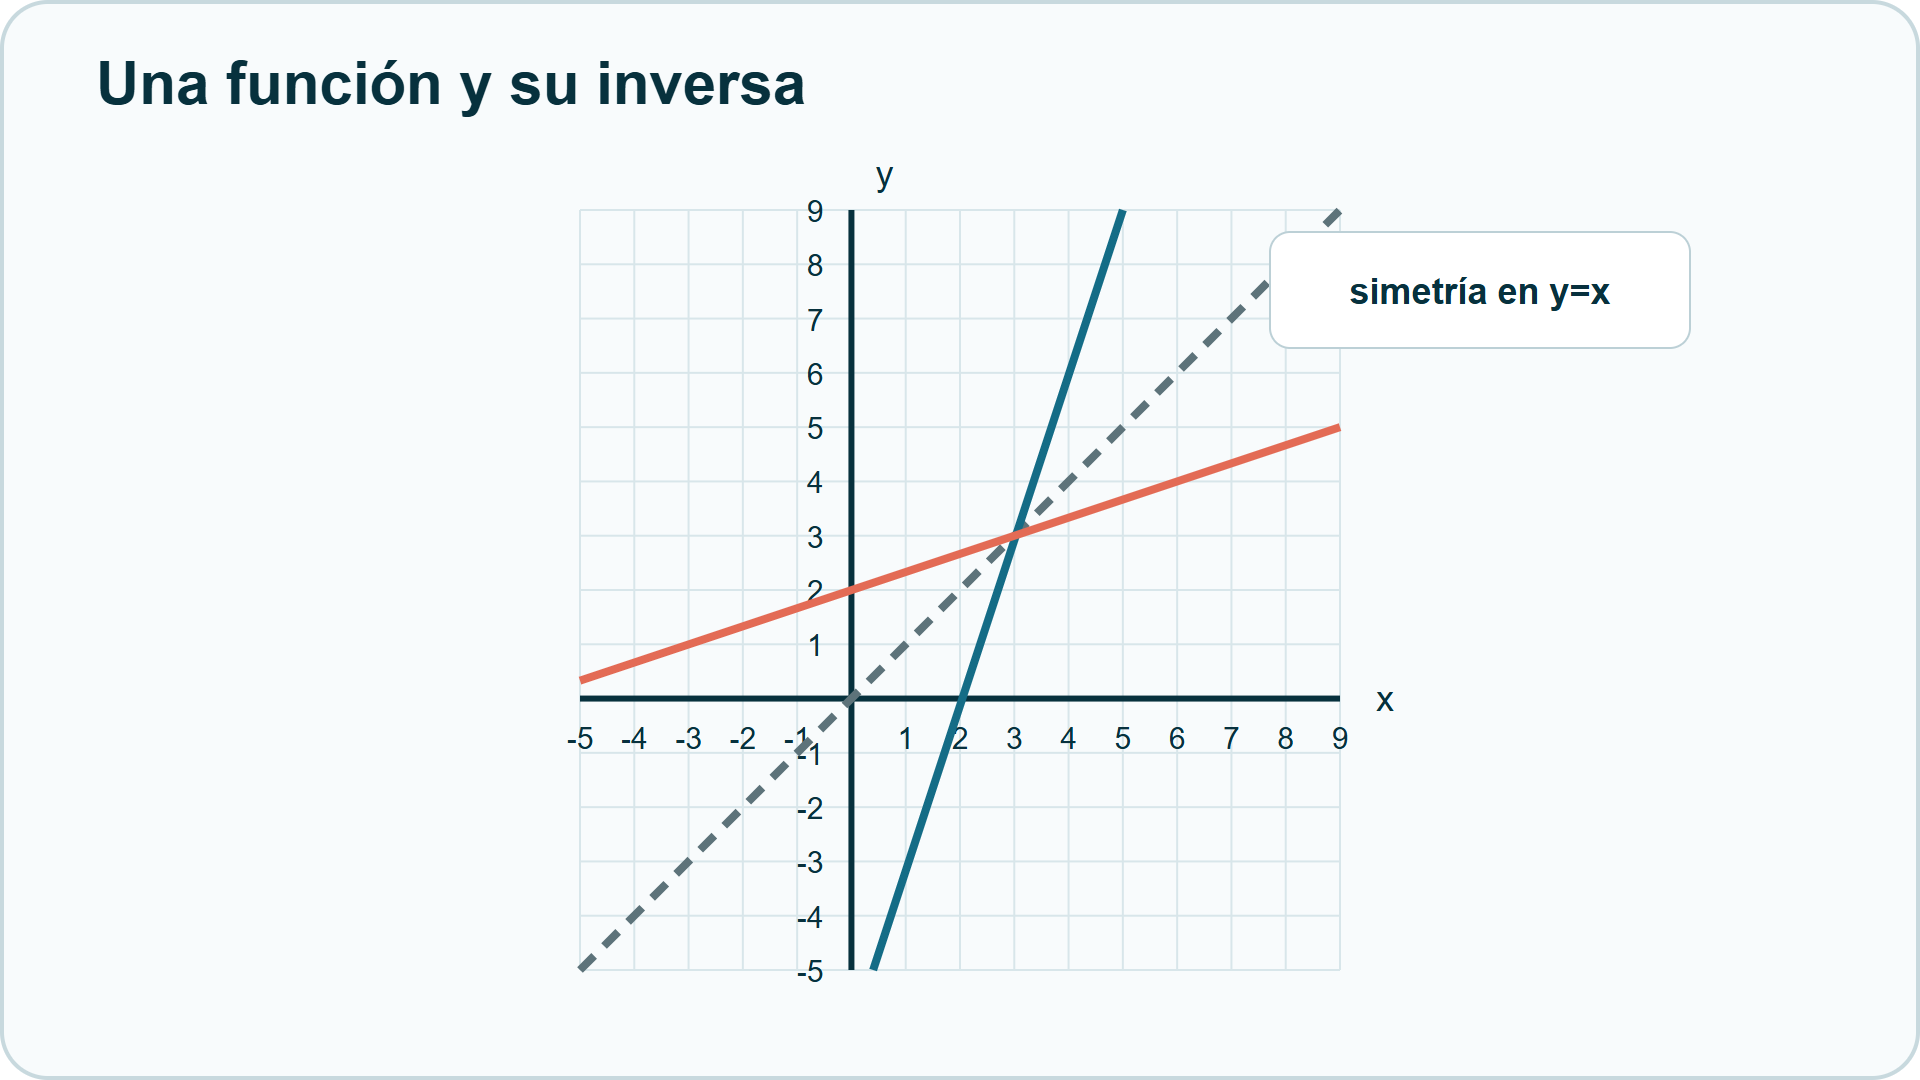
\includegraphics[width=0.80\linewidth,height=0.27\textheight,keepaspectratio]{diagrama-4557f22084d5a6.png}
\end{center}

\textbf{Respuesta.} $f^{-1}(x)=\frac{x+6}{3}$.

\textbf{Pista.} Escribe $y=3x-6$, intercambia $x$ y $y$, y despeja $y$.

\textbf{Explicación.} Después de intercambiar: $x=3y-6$. Entonces $x+6=3y$ y $y=\frac{x+6}{3}$. Las gráficas de $f$ y $f^{-1}$ son simétricas respecto a $y=x$.


\vspace{0.8em}
\hrule
\vspace{1.1em}



\clearpage
\section*{Álgebra y modelos}
\addcontentsline{toc}{section}{Álgebra y modelos}

\subsection*{\textcolor{DeepBlue}{Álgebra y modelos} \hfill \$100}
\textbf{Pregunta.} La tabla muestra una relación entre $t$ y $y$. Determina el modelo algebraico.

\begin{center}
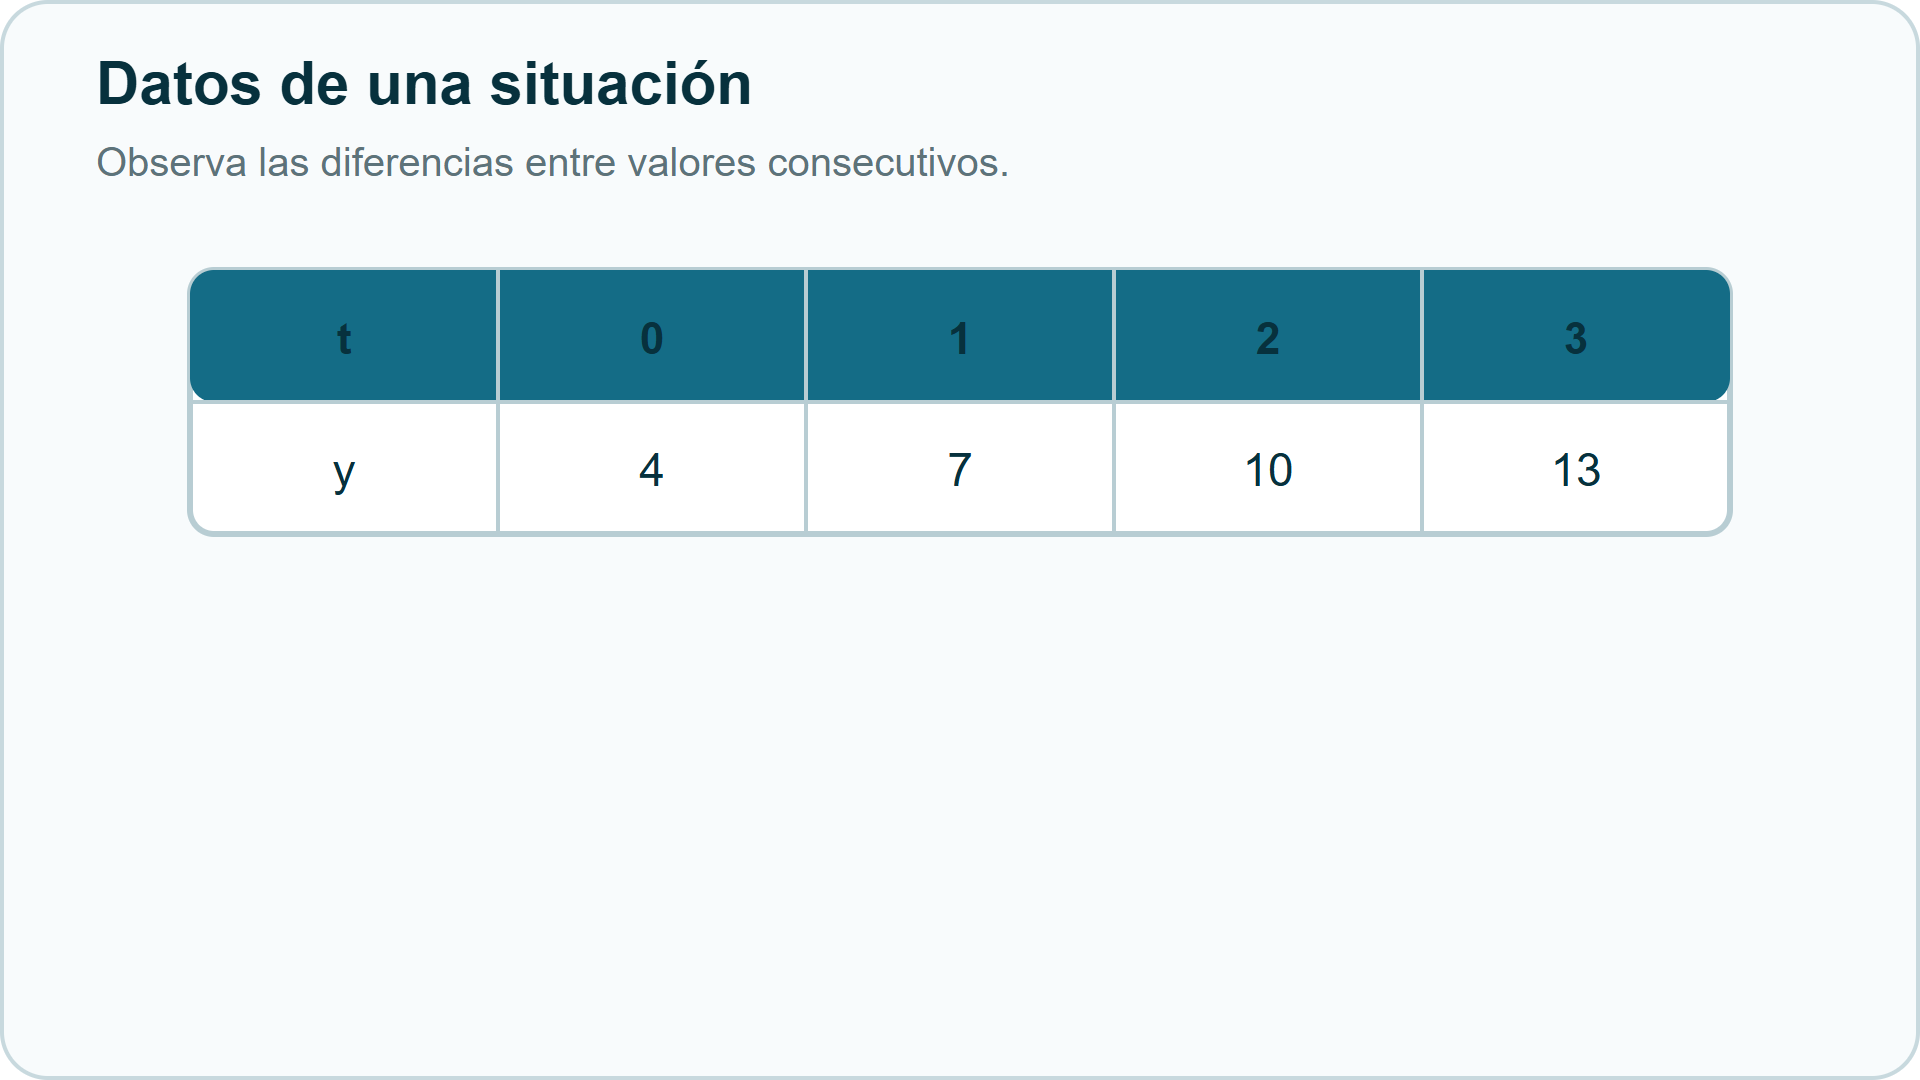
\includegraphics[width=0.80\linewidth,height=0.27\textheight,keepaspectratio]{diagrama-20a6f2397aec15.png}
\end{center}

\textbf{Respuesta.} $y=3t+4$.

\textbf{Pista.} Las diferencias de $y$ son constantes.

\textbf{Explicación.} Cada vez que $t$ aumenta $1$, $y$ aumenta $3$, así que la pendiente es $3$. Cuando $t=0$, $y=4$, por lo que el modelo es $y=3t+4$.


\vspace{0.8em}
\hrule
\vspace{1.1em}


\subsection*{\textcolor{DeepBlue}{Álgebra y modelos} \hfill \$200}
\textbf{Pregunta.} La población de la tabla aumenta con un patrón constante. Identifica el tipo de modelo y calcula $P(4)$.

\begin{center}
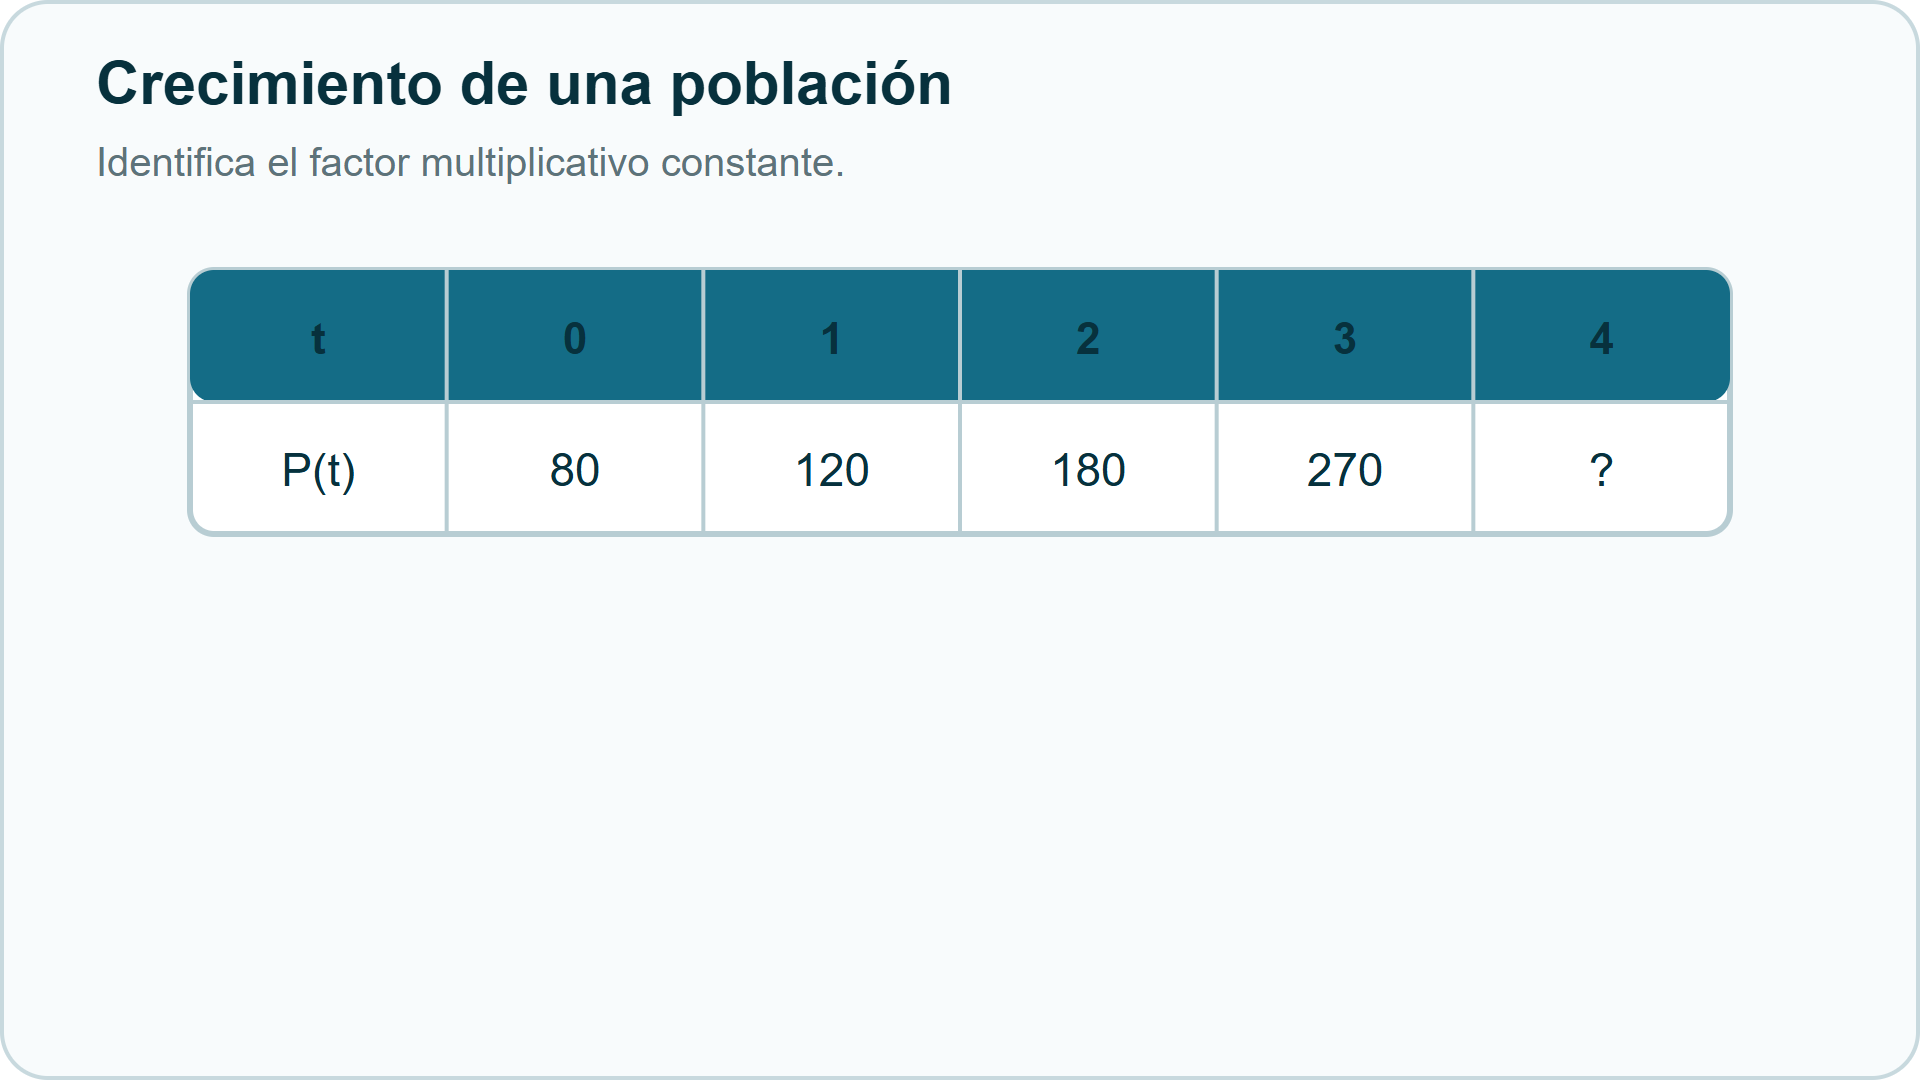
\includegraphics[width=0.80\linewidth,height=0.27\textheight,keepaspectratio]{diagrama-0012d9119b362e.png}
\end{center}

\textbf{Respuesta.} Modelo exponencial; $P(t)=80(1{,}5)^t$ y $P(4)=405$.

\textbf{Pista.} Divide cada valor entre el anterior.

\textbf{Explicación.} Los cocientes son $120/80=180/120=270/180=1{,}5$. El factor constante indica crecimiento exponencial. Luego, $270\times1{,}5=405$.


\vspace{0.8em}
\hrule
\vspace{1.1em}


\subsection*{\textcolor{DeepBlue}{Álgebra y modelos} \hfill \$300}
\textbf{Pregunta.} Para $d(t)=2\sqrt{t-1}+3$, indica el dominio y el valor inicial de la función.


\textbf{Respuesta.} Dominio $t\ge1$ y valor inicial $d(1)=3$.

\textbf{Pista.} El radicando debe ser no negativo.

\textbf{Explicación.} $t-1\ge0$ implica $t\ge1$. En el extremo del dominio, $d(1)=2\sqrt0+3=3$.

\begin{center}
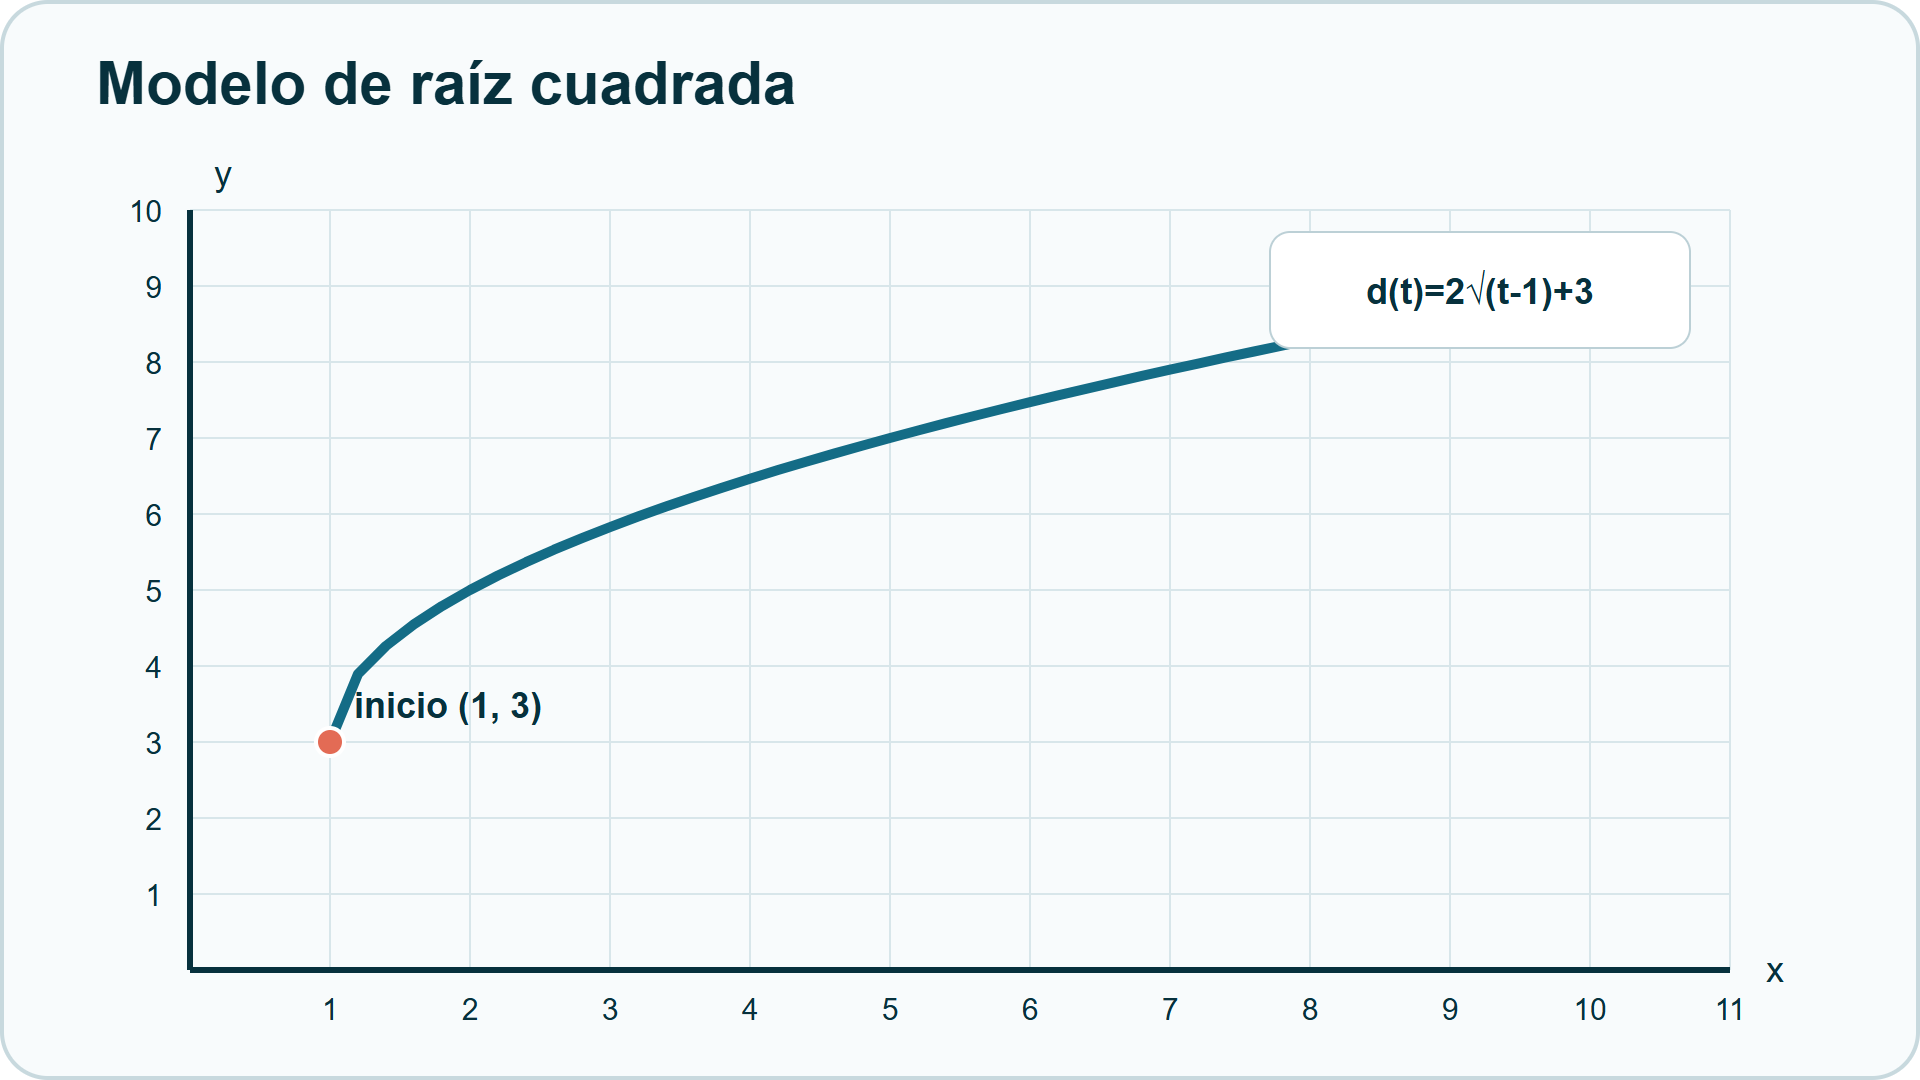
\includegraphics[width=0.80\linewidth,height=0.27\textheight,keepaspectratio]{diagrama-ff4fe29272443a.png}
\end{center}

\vspace{0.8em}
\hrule
\vspace{1.1em}


\subsection*{\textcolor{DeepBlue}{Álgebra y modelos} \hfill \$400}
\textbf{Pregunta.} Sean $f(x)=2x+1$ y $g(x)=\sqrt{x+1}$. Calcula $(f\circ g)(3)$.

\begin{center}
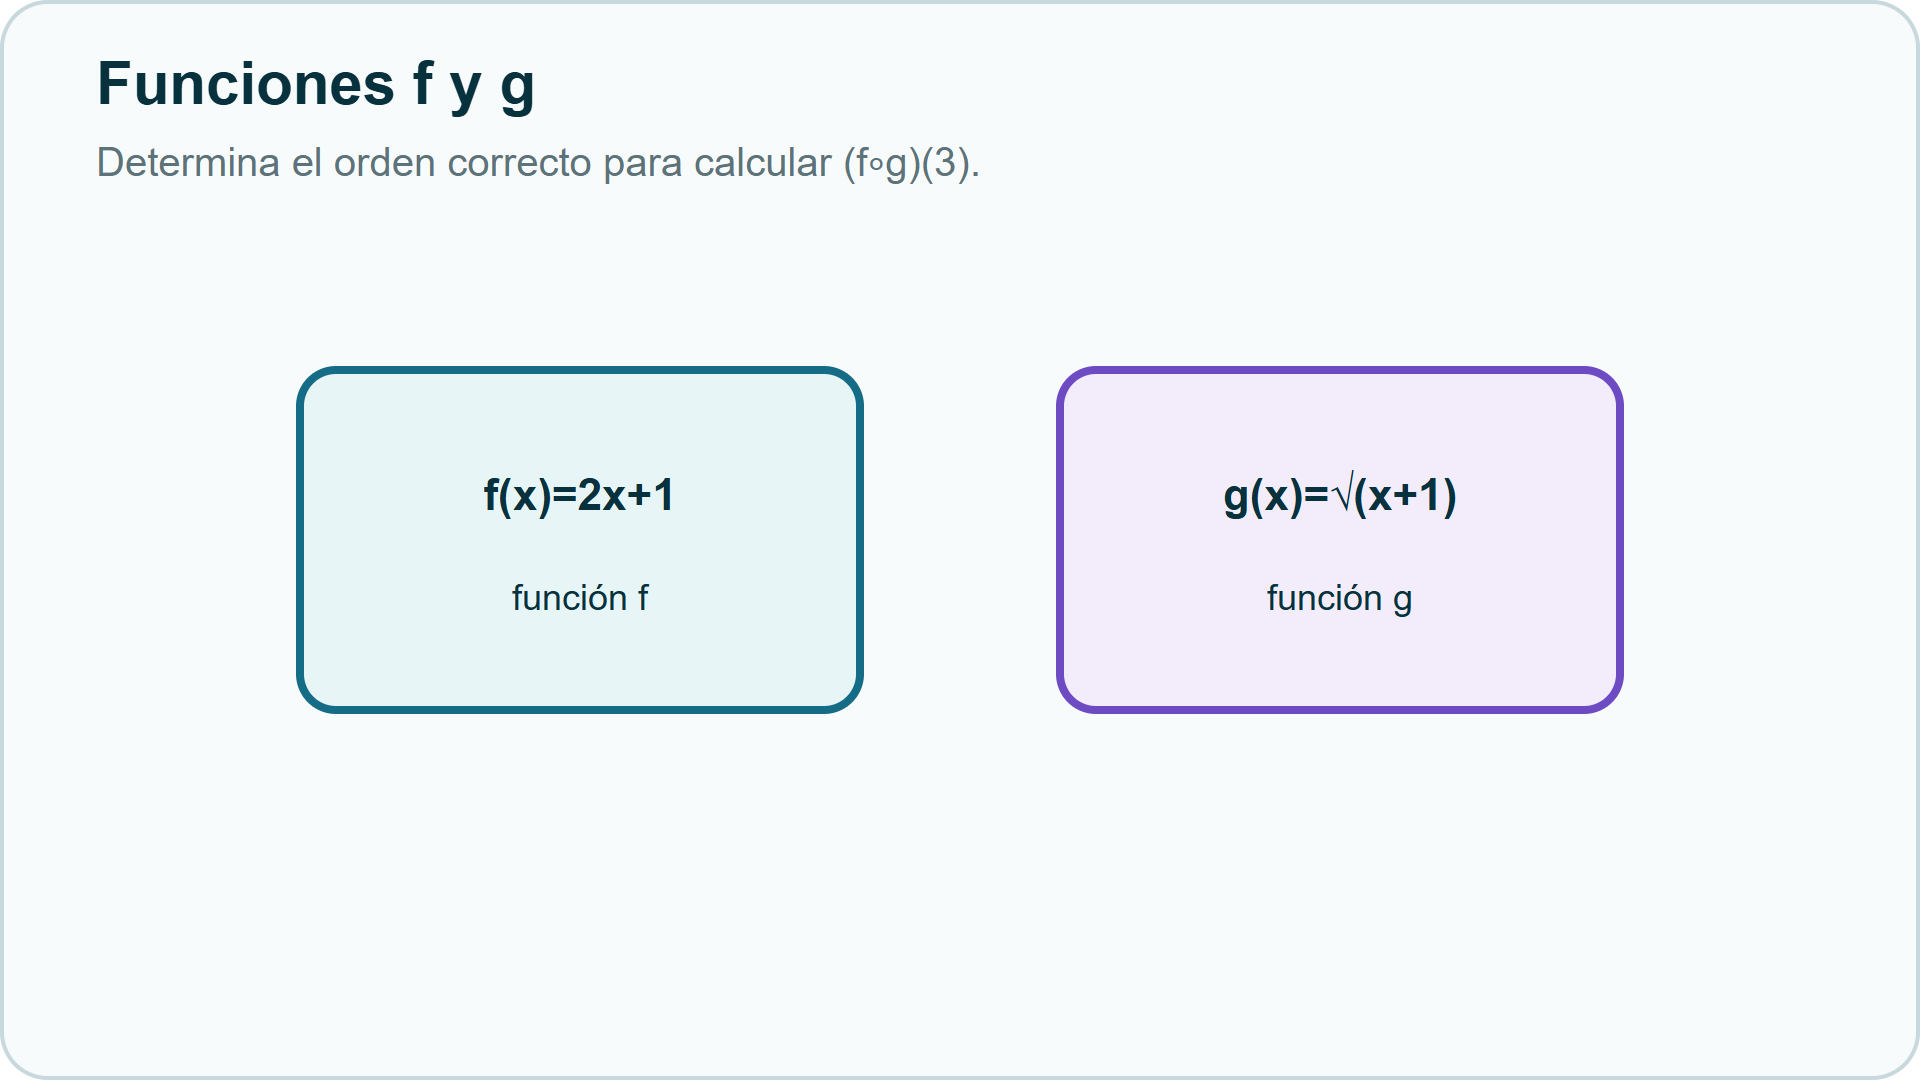
\includegraphics[width=0.80\linewidth,height=0.27\textheight,keepaspectratio]{diagrama-7a155396a603e1.png}
\end{center}

\textbf{Respuesta.} $(f\circ g)(3)=5$.

\textbf{Pista.} Primero calcula $g(3)$ y usa ese resultado como entrada de $f$.

\textbf{Explicación.} $g(3)=\sqrt{4}=2$. Luego, $f(2)=2(2)+1=5$.

\begin{center}
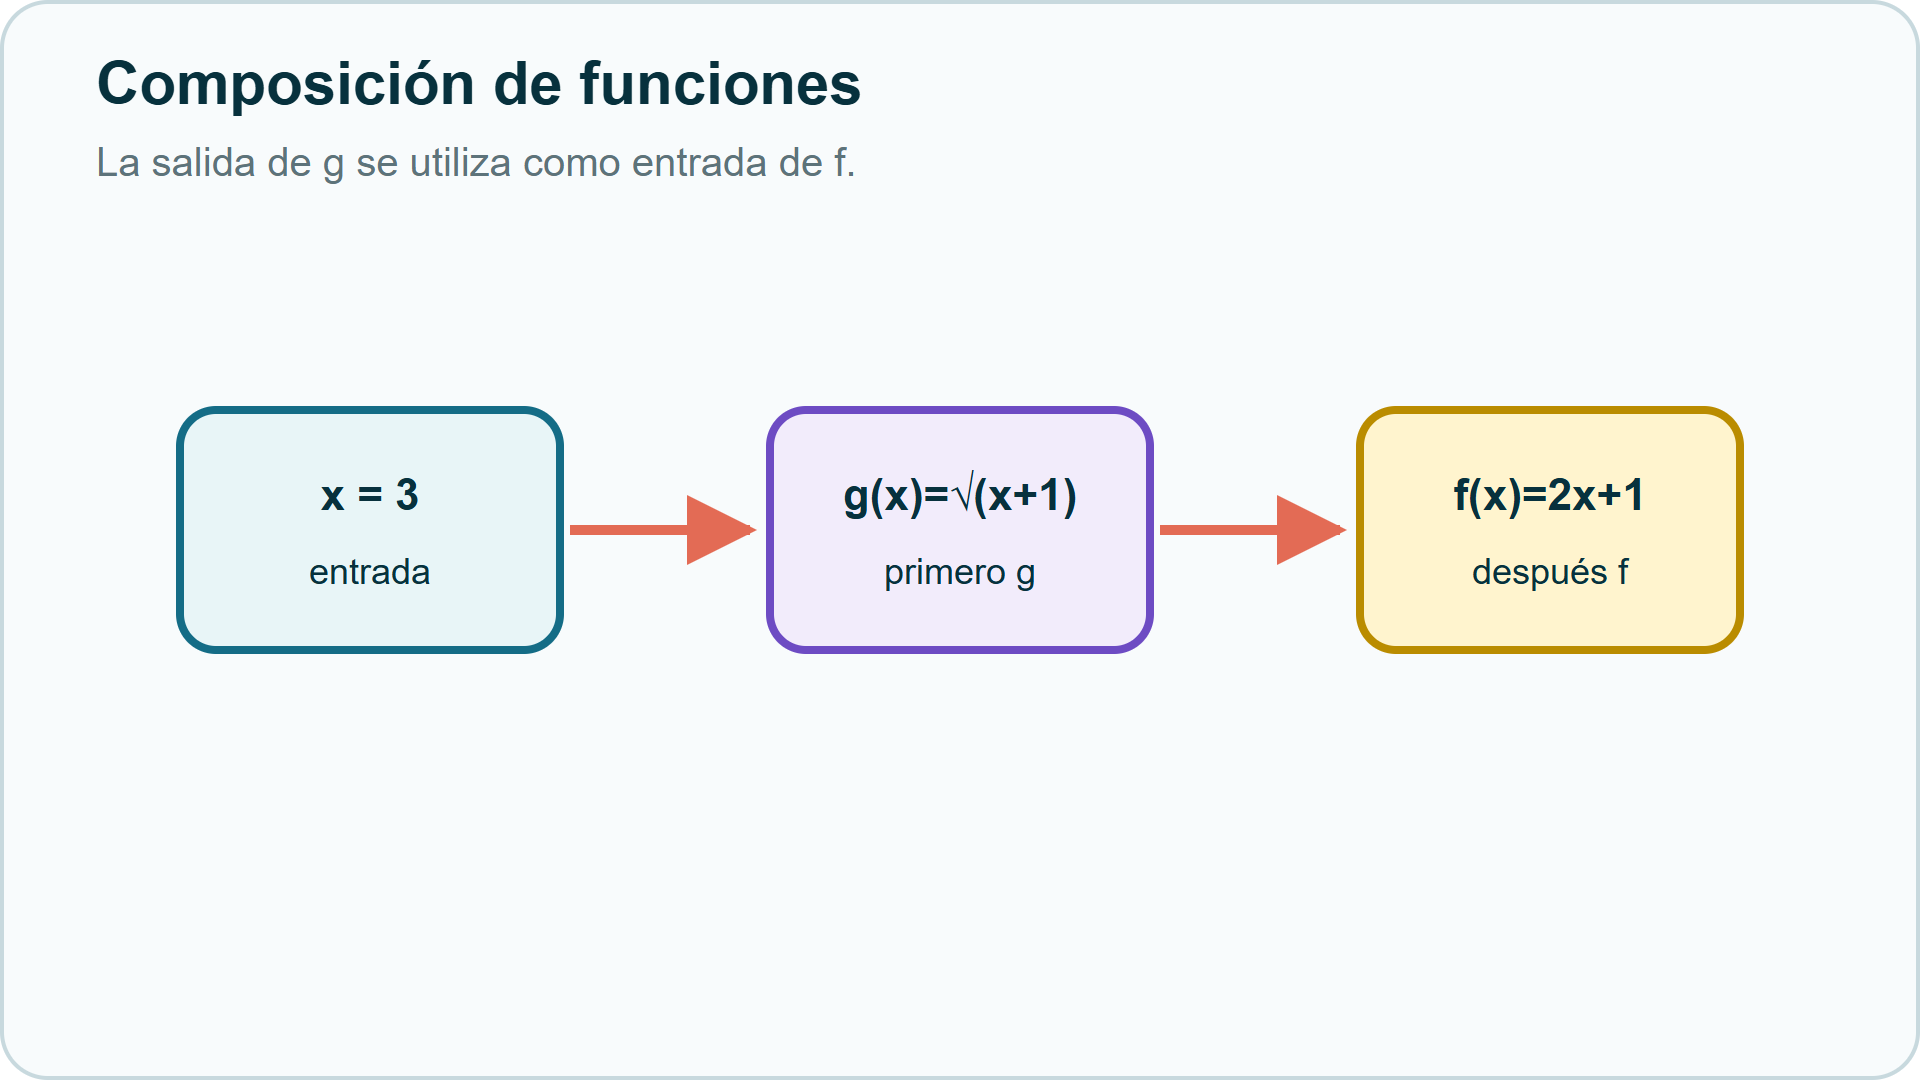
\includegraphics[width=0.80\linewidth,height=0.27\textheight,keepaspectratio]{diagrama-d69d347b4c263b.png}
\end{center}

\vspace{0.8em}
\hrule
\vspace{1.1em}


\subsection*{\textcolor{DeepBlue}{Álgebra y modelos} \hfill \$500}
\textbf{Pregunta.} Resuelve $\log_3(x)+\log_3(x-2)=1$.


\textbf{Respuesta.} $x=3$.

\textbf{Pista.} Combina los logaritmos y recuerda que $x>2$.

\textbf{Explicación.} $\log_3(x(x-2))=1$ implica $x(x-2)=3$. Entonces $x^2-2x-3=0$, es decir, $(x-3)(x+1)=0$. Solo $x=3$ cumple el dominio $x>2$.


\vspace{0.8em}
\hrule
\vspace{1.1em}



\clearpage
\section*{Estadística y azar}
\addcontentsline{toc}{section}{Estadística y azar}

\subsection*{\textcolor{DeepBlue}{Estadística y azar} \hfill \$100}
\textbf{Pregunta.} Para los datos $4,5,5,7,9$, determina la mediana, la moda y el recorrido.


\textbf{Respuesta.} Mediana $5$, moda $5$ y recorrido $5$.

\textbf{Pista.} Los datos ya están ordenados; el recorrido es máximo menos mínimo.

\textbf{Explicación.} El valor central es $5$, el valor que más se repite es $5$ y $9-4=5$.


\vspace{0.8em}
\hrule
\vspace{1.1em}


\subsection*{\textcolor{DeepBlue}{Estadística y azar} \hfill \$200}
\textbf{Pregunta.} Una calificación se compone de $30\%$ de tareas ($70$), $30\%$ de proyecto ($85$) y $40\%$ de prueba ($90$). Calcula la nota ponderada.


\textbf{Respuesta.} $82{,}5$.

\textbf{Pista.} Multiplica cada nota por su peso decimal y suma.

\textbf{Explicación.} $70(0{,}30)+85(0{,}30)+90(0{,}40)=21+25{,}5+36=82{,}5$.


\vspace{0.8em}
\hrule
\vspace{1.1em}


\subsection*{\textcolor{DeepBlue}{Estadística y azar} \hfill \$300}
\textbf{Pregunta.} En el diagrama, $P(A)=0{,}55$, $P(B)=0{,}40$ y $P(A\cap B)=0{,}20$. Calcula $P(A\cup B)$ y $P(A^c)$.

\begin{center}
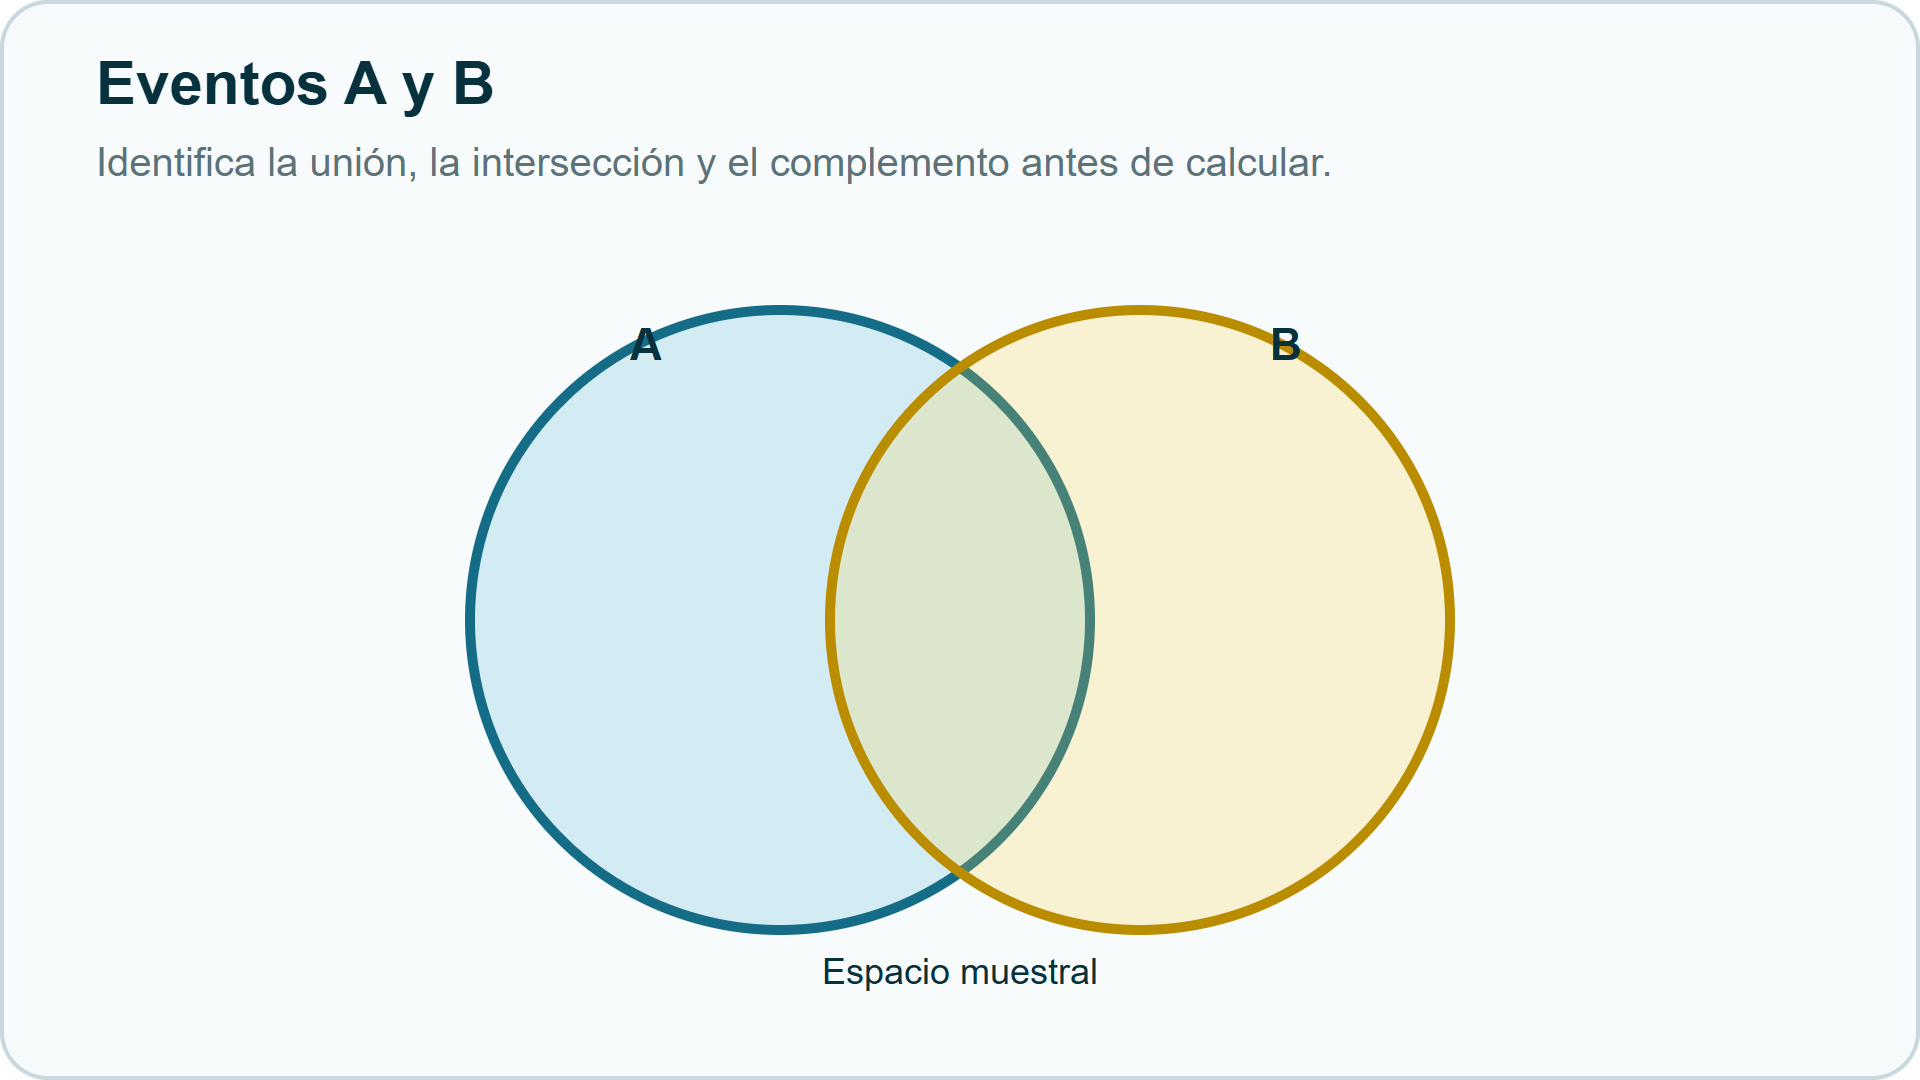
\includegraphics[width=0.80\linewidth,height=0.27\textheight,keepaspectratio]{diagrama-121d1191fb1a59.png}
\end{center}

\textbf{Respuesta.} $P(A\cup B)=0{,}75$ y $P(A^c)=0{,}45$.

\textbf{Pista.} En la unión, resta una vez la intersección; para el complemento, resta de $1$.

\textbf{Explicación.} $P(A\cup B)=0{,}55+0{,}40-0{,}20=0{,}75$. Además, $P(A^c)=1-0{,}55=0{,}45$.

\begin{center}
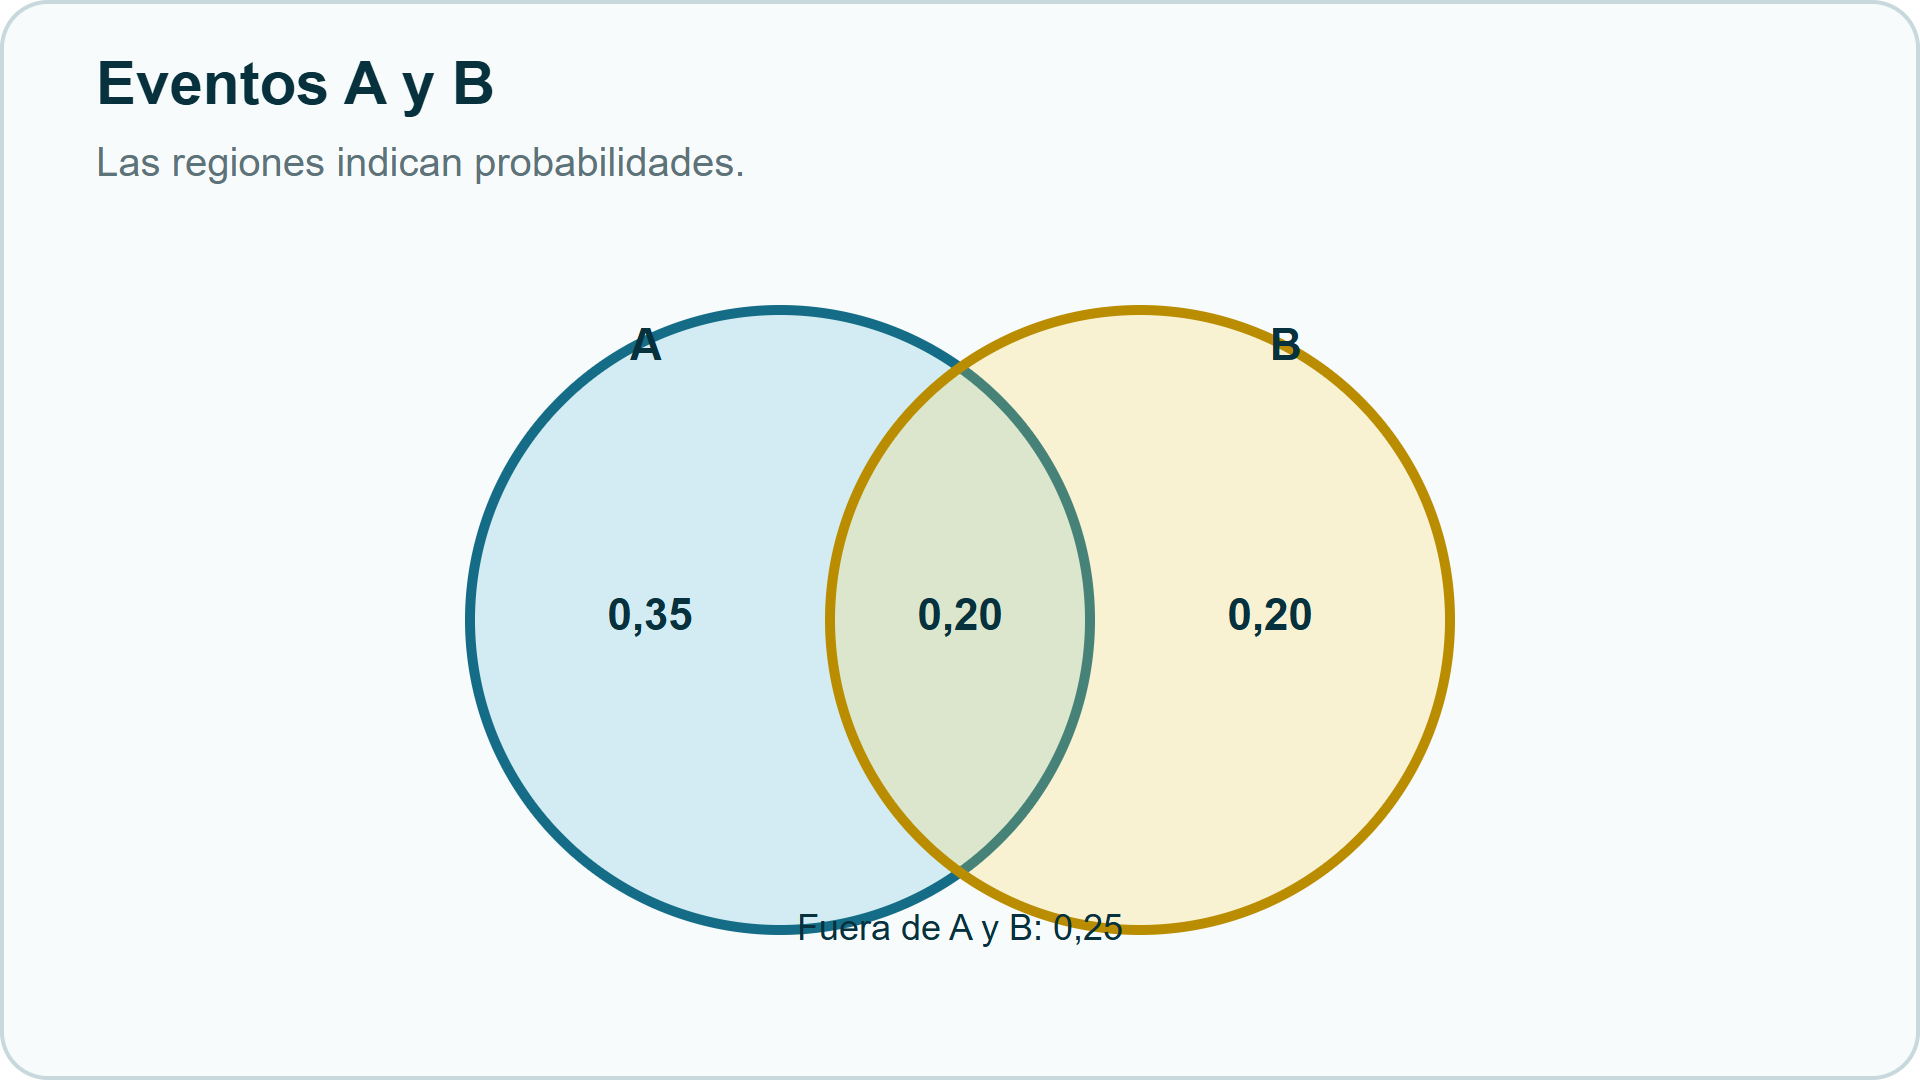
\includegraphics[width=0.80\linewidth,height=0.27\textheight,keepaspectratio]{diagrama-34ba932dac7196.png}
\end{center}

\vspace{0.8em}
\hrule
\vspace{1.1em}


\subsection*{\textcolor{DeepBlue}{Estadística y azar} \hfill \$400}
\textbf{Pregunta.} Observa los diagramas de cajas. ¿Cuál grupo tiene mayor mediana y cuál tiene mayor recorrido intercuartílico?

\begin{center}
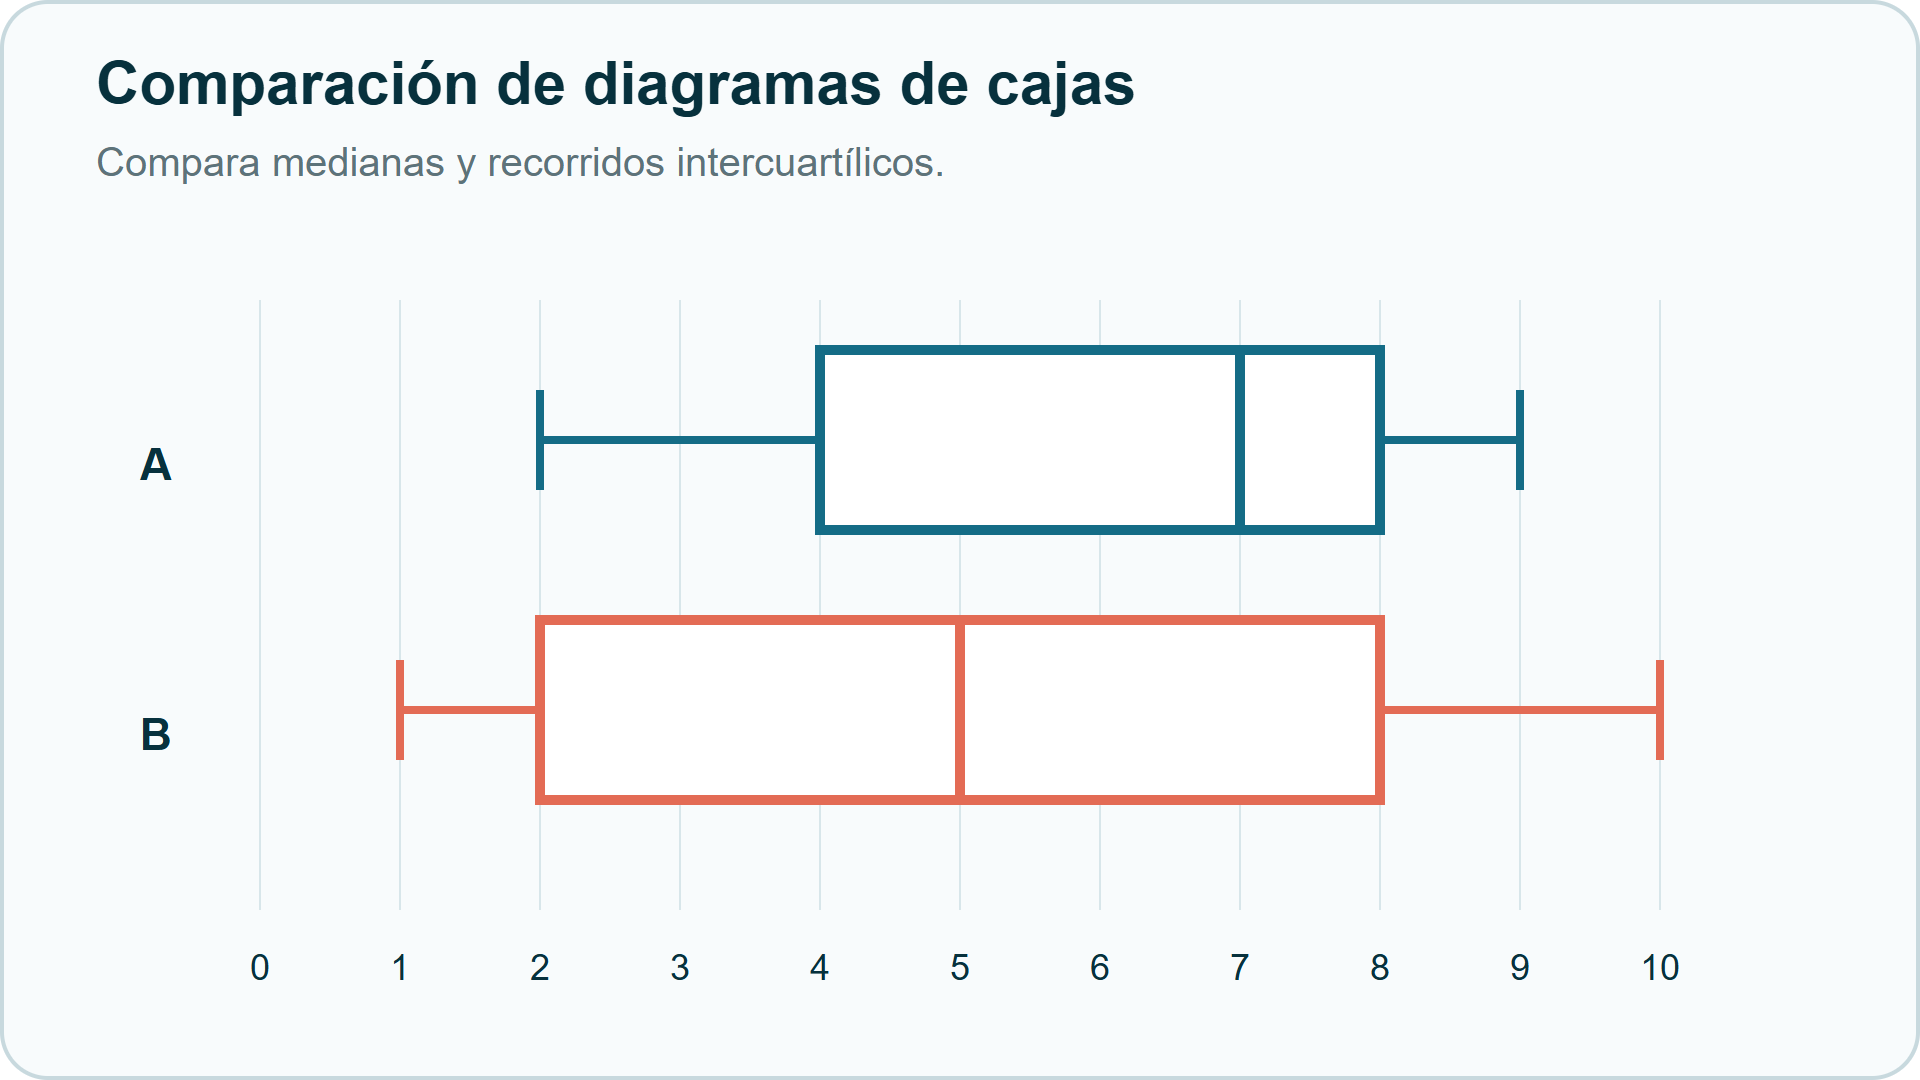
\includegraphics[width=0.80\linewidth,height=0.27\textheight,keepaspectratio]{diagrama-b5410e5e34eb61.png}
\end{center}

\textbf{Respuesta.} El grupo A tiene mayor mediana y el grupo B tiene mayor recorrido intercuartílico.

\textbf{Pista.} La mediana es la línea dentro de la caja; el RIC es el ancho de la caja.

\textbf{Explicación.} En A, la mediana es $7$ y el RIC es $8-4=4$. En B, la mediana es $5$ y el RIC es $8-2=6$. Por eso A tiene mayor mediana, mientras que B tiene mayor dispersión central.


\vspace{0.8em}
\hrule
\vspace{1.1em}


\subsection*{\textcolor{DeepBlue}{Estadística y azar} \hfill \$500}
\textbf{Pregunta.} El grupo X tiene media $80$ y desviación estándar $8$; el grupo Y tiene media $50$ y desviación estándar $7{,}5$. ¿Cuál presenta mayor variabilidad relativa?

\begin{center}
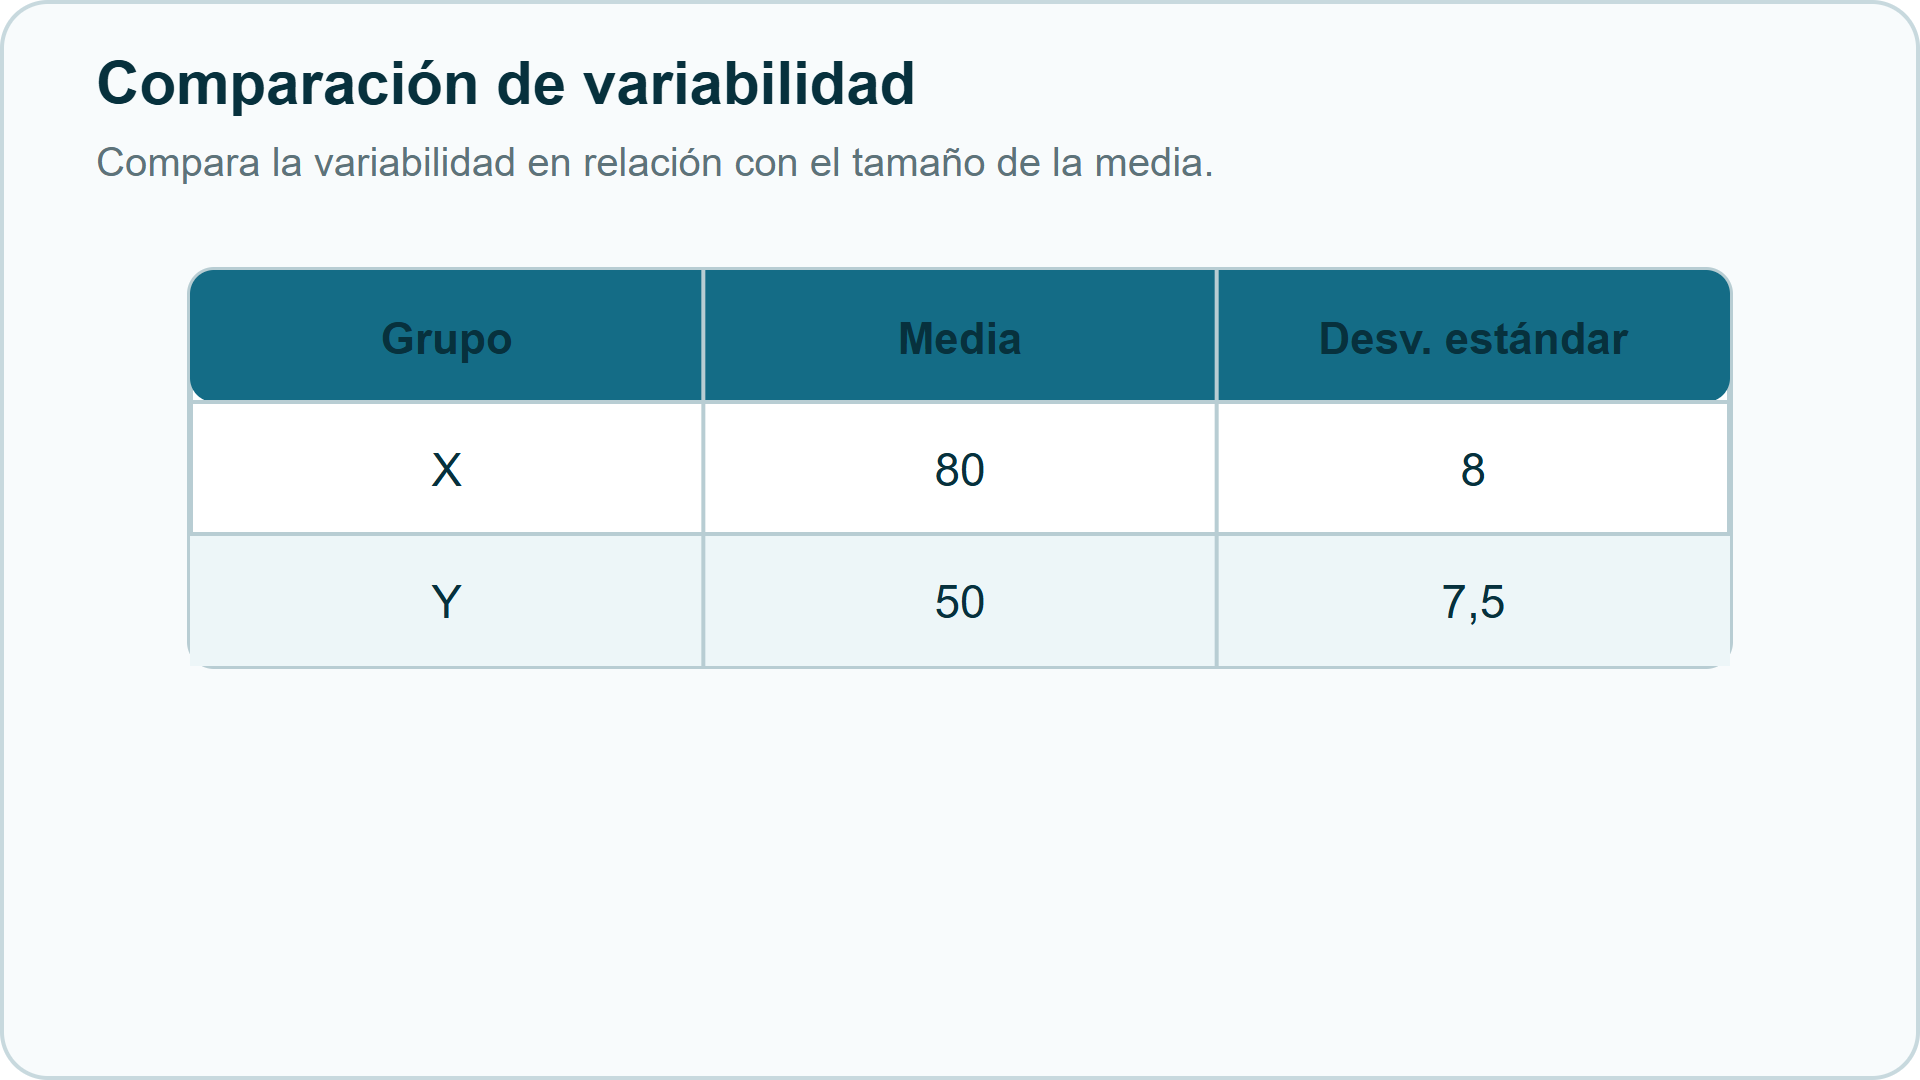
\includegraphics[width=0.80\linewidth,height=0.27\textheight,keepaspectratio]{diagrama-b24dfac2b3a543.png}
\end{center}

\textbf{Respuesta.} El grupo Y.

\textbf{Pista.} Compara los coeficientes de variación $CV=\frac{s}{\bar{x}}\times100\%$.

\textbf{Explicación.} Para X, $CV=\frac8{80}\times100\%=10\%$. Para Y, $CV=\frac{7{,}5}{50}\times100\%=15\%$. Por eso Y tiene mayor variabilidad relativa.


\vspace{0.8em}
\hrule
\vspace{1.1em}



\clearpage
\section*{Reto final: Geometría analítica}
\addcontentsline{toc}{section}{Reto final}
\subsection*{\textcolor{DeepBlue}{Reto final} \hfill Apuesta libre}
\textbf{Pregunta.} Un jardín circular tiene centro $C(2,-1)$ y pasa por $P(5,3)$. Determina la ecuación de la circunferencia y una ecuación de la recta tangente en $P$.

\begin{center}
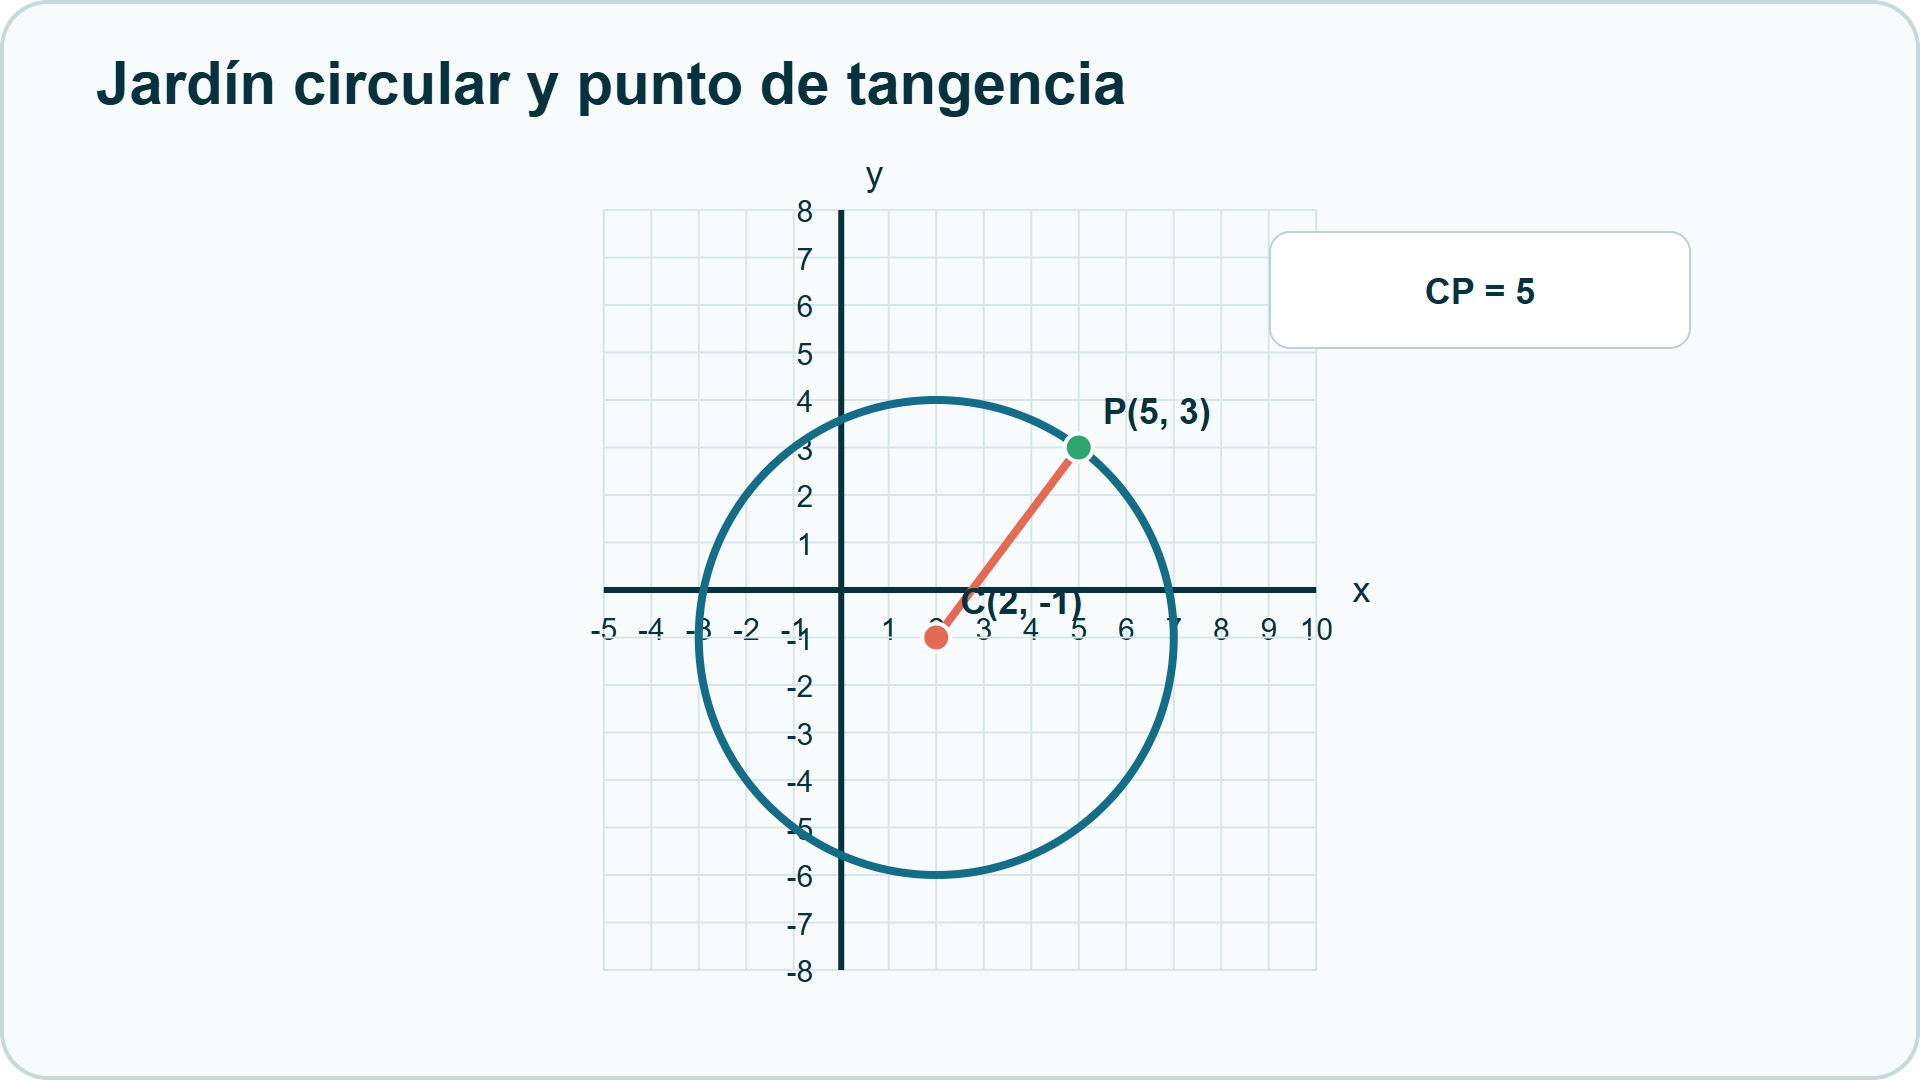
\includegraphics[width=0.80\linewidth,height=0.27\textheight,keepaspectratio]{diagrama-832fc0be01e3cb.png}
\end{center}

\textbf{Respuesta.} Circunferencia: $(x-2)^2+(y+1)^2=25$. Tangente: $y-3=-\frac{3}{4}(x-5)$.

\textbf{Explicación.} El radio $\overline{CP}$ tiene vector $(3,4)$, longitud $5$ y pendiente $\frac{4}{3}$. La tangente es perpendicular, por lo que su pendiente es $-\frac{3}{4}$ y pasa por $P(5,3)$.

\begin{center}
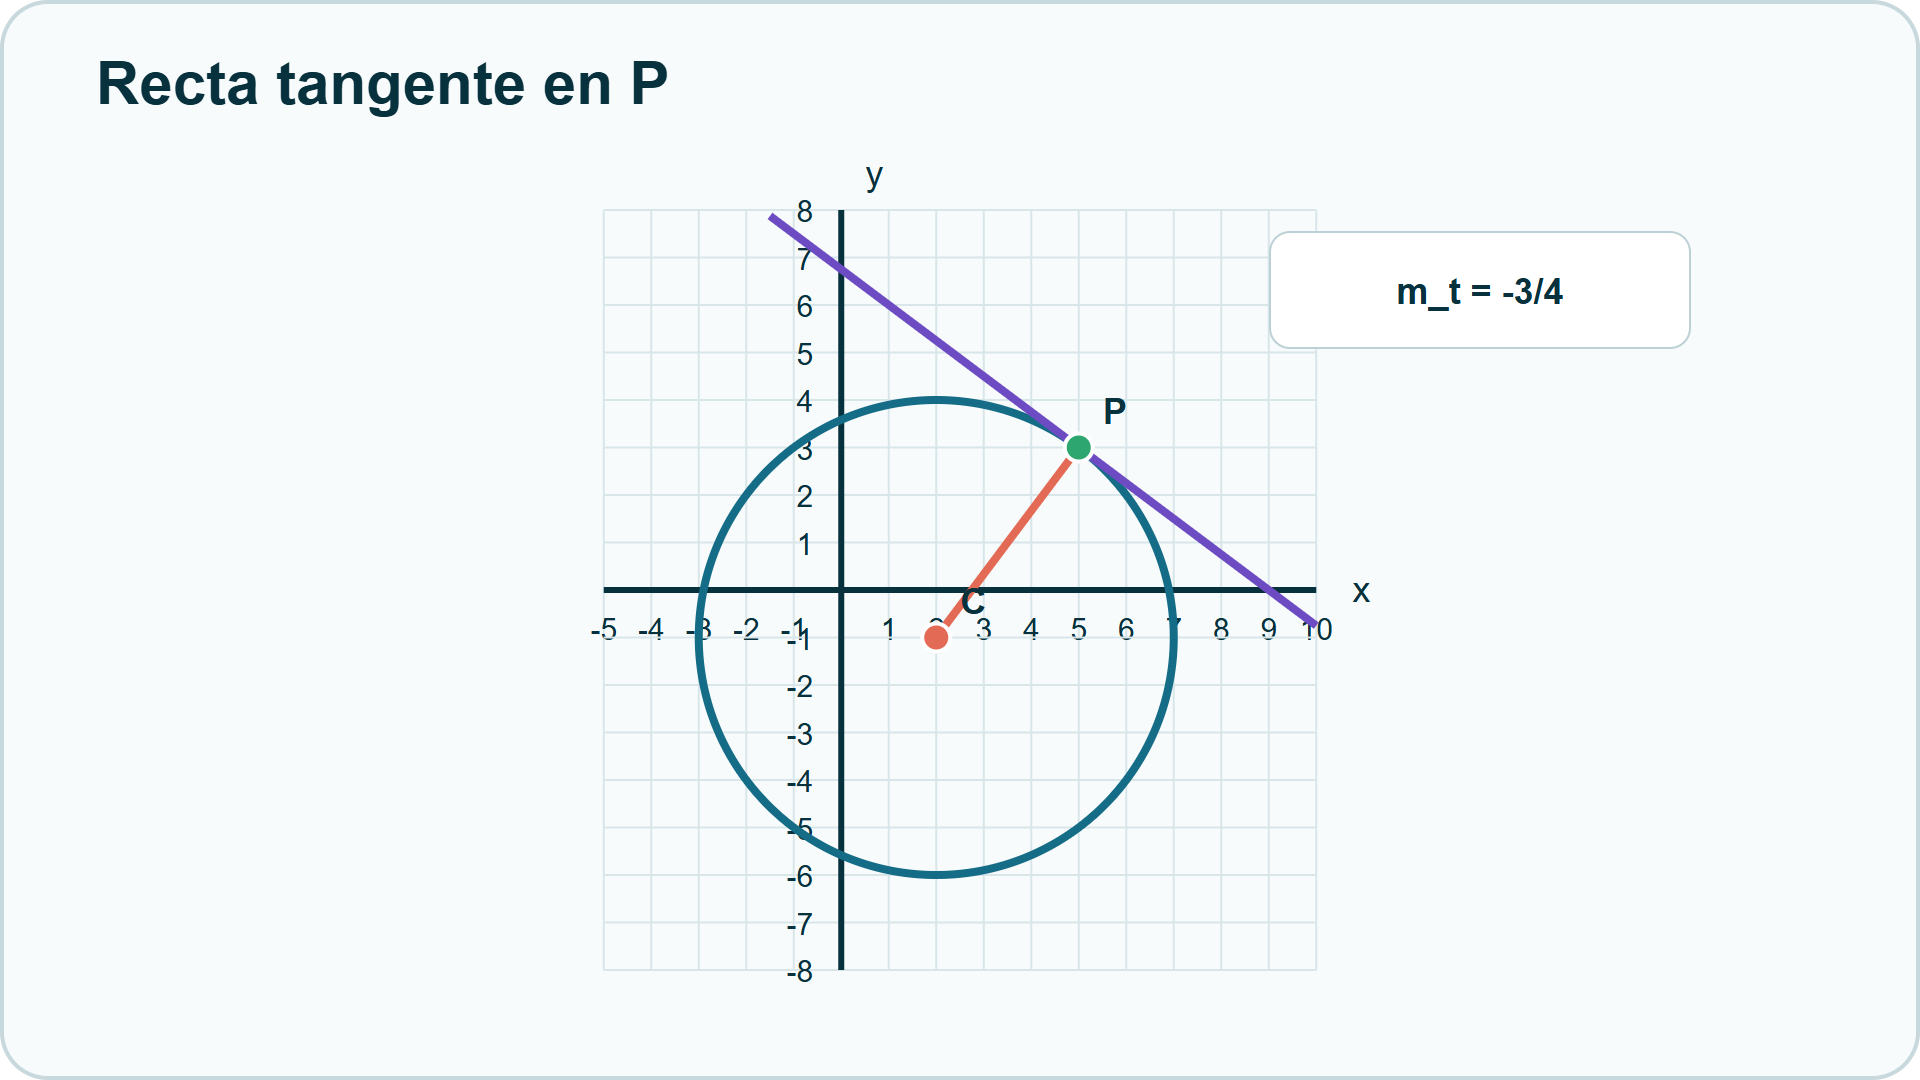
\includegraphics[width=0.80\linewidth,height=0.27\textheight,keepaspectratio]{diagrama-eaad5649a2749e.png}
\end{center}

\end{document}
